%%%%%%%%%%%%%%%%%%%%%%%%%%%%%%%%%%%%%%%%%
% Masters/Doctoral Thesis 
% LaTeX Template
% Version 1.43 (17/5/14)
%
% This template has been downloaded from:
% http://www.LaTeXTemplates.com
%
% Original authors:
% Steven Gunn 
% http://users.ecs.soton.ac.uk/srg/softwaretools/document/templates/
% and
% Sunil Patel
% http://www.sunilpatel.co.uk/thesis-template/
%
% License:
% CC BY-NC-SA 3.0 (http://creativecommons.org/licenses/by-nc-sa/3.0/)
%
% Note:
% Make sure to edit document variables in the Thesis.cls file
%
%%%%%%%%%%%%%%%%%%%%%%%%%%%%%%%%%%%%%%%%%

%-------------------------------------------------------------------------------
%	PACKAGES AND OTHER DOCUMENT CONFIGURATIONS
%-------------------------------------------------------------------------------

\documentclass[12pt, twosides]{Thesis} % The default font size and one-sided printing (no margin offsets)

\graphicspath{{Pictures/}} % Specifies the directory where pictures are stored
\usepackage[square, numbers, comma, sort&compress]{natbib} % Use the natbib reference package - read up on this to edit the reference style; if you want text (e.g. Smith et al., 2012) for the in-text references (instead of numbers), remove 'numbers' 
\usepackage{subfig}
\usepackage{graphicx}
\usepackage{float}
\usepackage{caption}
\usepackage{pst-all}
\usepackage{amsmath}
\usepackage{mathtools}
\usepackage{amsfonts}
\usepackage{soul}
\usepackage{listings}
\usepackage{color}
\usepackage{tabularx}
\usepackage{nicefrac}
\usepackage{moresize}
\usepackage[italian]{babel}
\captionsetup[figure]{name=Figura}
\hypersetup{urlcolor=black, colorlinks=true} % Colors hyperlinks in blue - change to black if annoying
\title{\ttitle} % Defines the thesis title - don't touch this
\setcounter{tocdepth}{3}
\begin{document}

\frontmatter % Use roman page numbering style (i, ii, iii, iv...) for the pre-content pages

\setstretch{1.3} % Line spacing of 1.3

% Define the page headers using the FancyHdr package and set up for one-sided printing
\fancyhead{} % Clears all page headers and footers
\rhead{\thepage} % Sets the right side header to show the page number
\lhead{} % Clears the left side page header

\pagestyle{fancy} % Finally, use the "fancy" page style to implement the FancyHdr headers

\newcommand{\HRule}{\rule{\linewidth}{0.5mm}} % New command to make the lines in the title page
% PDF meta-data
\hypersetup{pdftitle={\ttitle}}
\hypersetup{pdfsubject=\subjectname}
\hypersetup{pdfauthor=\iauthors}
\hypersetup{pdfkeywords=\keywordnames}

%-------------------------------------------------------------------------------
%	TITLE PAGE
%-------------------------------------------------------------------------------

\begin{titlepage}
\begin{center}

%\textsc{\LARGE \univname}\\[1.5cm] % University name

\includegraphics[width=9.98cm,height=6.1cm]{Figures/UNIGE.jpg}\\[1cm]

\textsc{\Large \textbf{Tesi di Laurea}}\\[0.5cm] % Thesis type

\HRule \\[0.4cm] % Horizontal line
{\huge \bfseries \ttitle}\\[0.4cm] % Thesis title
\HRule \\[1.0cm] % Horizontal line
 
\begin{minipage}{0.45\textwidth}
\begin{flushleft} \large
\emph{Relatore:} \\
\href{http://goo.gl/JQlltW}{\supname} \\ % Supervisor name - remove the \href 
%bracket to remove the link  
\emph{Correlatore:} \\
{\crelator}
\end{flushleft}
\end{minipage}
\begin{minipage}{0.45\textwidth}
\begin{flushright} \large\emph{Candidati:}\\
{\nauthors} % Author name - remove the \href bracket to remove the link
\end{flushright}
\end{minipage}\\[1.2cm]
 
\textit{A thesis submitted in fulfilment of the requirements\\ for the 
degree of \degreename}\\[.3cm] % University requirement text
\textit{in the}\\[.4cm]
\groupname\\\deptname\\[.5cm] % Research group name and department name
 
{\today}\\[4cm] % Date
%\includegraphics{Logo} % University/department logo - uncomment to place it
 
\vfill
\end{center}

\end{titlepage}

%-------------------------------------------------------------------------------
%	DECLARATION PAGE
%	Your institution may give you a different text to place here
%-------------------------------------------------------------------------------

\Declaration{

\addtocontents{toc}{\vspace{1em}} % Add a gap in the Contents, for aesthetics

I, \iauthors, declare that this thesis titled, '\ttitle' and the work presented in it are my own. I confirm that:

\begin{itemize} 
\item[\tiny{$\blacksquare$}] This work was done wholly or mainly while in candidature for a research degree at this University.
\item[\tiny{$\blacksquare$}] Where any part of this thesis has previously been submitted for a degree or any other qualification at this University or any other institution, this has been clearly stated.
\item[\tiny{$\blacksquare$}] Where I have consulted the published work of others, this is always clearly attributed.
\item[\tiny{$\blacksquare$}] Where I have quoted from the work of others, the source is always given. With the exception of such quotations, this thesis is entirely my own work.
\item[\tiny{$\blacksquare$}] I have acknowledged all main sources of help.
\item[\tiny{$\blacksquare$}] Where the thesis is based on work done by myself jointly with others, I have made clear exactly what was done by others and what I have contributed myself.\\
\end{itemize}
 
Signed:\\
\rule[1em]{25em}{0.5pt} % This prints a line for the signature
 
Date:\\
\rule[1em]{25em}{0.5pt} % This prints a line to write the date
}

\clearpage % Start a new page

%-------------------------------------------------------------------------------
%	QUOTATION PAGE
%-------------------------------------------------------------------------------

\pagestyle{empty} % No headers or footers for the following pages

\null\vfill % Add some space to move the quote down the page a bit    \renewcommand{\chaptername}{}

\textit{``Thanks to my solid academic training, today I can write hundreds of words on virtually any topic without possessing a shred of information, which is how I got a good job in journalism."}

\begin{flushright}
Dave Barry
\end{flushright}

\vfill\vfill\vfill\vfill\vfill\vfill\null % Add some space at the bottom to position the quote just right

\clearpage % Start a new page

%-------------------------------------------------------------------------------
%	ABSTRACT PAGE
%-------------------------------------------------------------------------------

\addtotoc{Abstract} % Add the "Abstract" page entry to the Contents

\abstract{\addtocontents{toc}{\vspace{1em}} % Add a gap in the Contents, for aesthetics

The Thesis Abstract is written here (and usually kept to just this page). The page is kept centered vertically so can expand into the blank space above the title too\ldots
}
\clearpage % Start a new page

%-------------------------------------------------------------------------------    \renewcommand{\chaptername}{}
%	ACKNOWLEDGEMENTS
%-------------------------------------------------------------------------------

\setstretch{1.3} % Reset the line-spacing to 1.3 for body text (if it has changed)

\acknowledgements{\addtocontents{toc}{\vspace{1em}} % Add a gap in the Contents, for aesthetics

The acknowledgements and the people to thank go here, don't forget to include your project advisor\ldots
}
\clearpage % Start a new page

%-------------------------------------------------------------------------------
%	LIST OF CONTENTS/FIGURES/TABLES PAGES
%-------------------------------------------------------------------------------

\pagestyle{fancy} % The page style headers have been "empty" all this time, now use the "fancy" headers as defined before to bring them back

\lhead{\emph{Indice}} % Set the left side page header to "Contents"
\tableofcontents % Write out the Table of Contents    \renewcommand{\chaptername}{}

\lhead{\emph{Elenco delle Figure}} % Set the left side page header to "List of Figures"
\listoffigures % Write out the List of Figures

\lhead{\emph{Elenco delle Tabelle}} % Set the left side page header to "List of Tables"
\listoftables % Write out the List of Tables

%-------------------------------------------------------------------------------
%	ABBREVIATIONS
%-------------------------------------------------------------------------------

\clearpage % Start a new page

\setstretch{1.5} % Set the line spacing to 1.5, this makes the following tables easier to read

\lhead{\emph{Acronimi}} % Set the left side page header to "Abbreviations"
\listofsymbols{ll} % Include a list of Abbreviations (a table of two columns)
{
  % A
  \textbf{ABS}   & \textbf{A}ntilock \textbf{B}raking \textbf{S}ystem \\
  \textbf{AMVP}  & \textbf{A}dvanced \textbf{M}otion \textbf{V}ector 
  \textbf{P}rediction \\
  
  % B
  \textbf{BO}    & \textbf{B}and \textbf{O}ffset \\
  
  % C
  \textbf{CABAC} & \textbf{C}ontext-based \textbf{A}daptive \textbf{B}inary
  \textbf{A}rithmetic \textbf{C}oding \\
  
  \textbf{CB}    & \textbf{C}oding \textbf{B}lock \\
  \textbf{CIF}   & \textbf{C}ommon \textbf{I}ntermediate \textbf{F}ormat \\
  \textbf{CISC}  & \textbf{C}omplex \textbf{I}nstruction \textbf{S}et 
  \textbf{C}omputing \\
  
  \textbf{CPSR}  & \textbf{C}urrent \textbf{P}rogram \textbf{S}tatus 
  \textbf{R}egister \\
  
  \textbf{CPU}   & \textbf{C}entral \textbf{P}rocessing \textbf{U}nit \\
  \textbf{CSE}   & \textbf{C}ommon \textbf{S}ubexpression \textbf{E}limination\\
  \textbf{CSI}   & \textbf{C}amera \textbf{S}ignal \textbf{I}nterface \\
  \textbf{CTB}   & \textbf{C}oding \textbf{T}ree \textbf{B}lock \\
  \textbf{CTU}   & \textbf{C}oding \textbf{T}ree \textbf{U}nit \\
  \textbf{CU}    & \textbf{C}oding \textbf{U}nit \\
  
  % D
  \textbf{DCT}   & \textbf{D}iscrete \textbf{C}osine \textbf{T}ransform \\
  \textbf{DDR}   & \textbf{D}ouble \textbf{D}ata \textbf{R}ate \\
  \textbf{DFT}   & \textbf{D}iscrete \textbf{F}ourier \textbf{T}ransform \\
  \textbf{DPCM}  & \textbf{D}ifferential \textbf{P}ulse-\textbf{C}ode 
  \textbf{M}odulation \\
  
  \textbf{DST}   & \textbf{D}iscrete \textbf{S}ine \textbf{T}ransform \\
  
  % E
  \textbf{EO}    & \textbf{E}dge \textbf{O}ffset \\
  
  % F
  \textbf{FTP}   & \textbf{F}ile \textbf{T}ransfer \textbf{P}rotocol \\
  
  % G
  \textbf{GCC}   & \textbf{G}NU \textbf{C}ompiler \textbf{C}ollection \\
  \textbf{GOP}   & \textbf{G}roup \textbf{O}f \textbf{P}ictures \\
  \textbf{GPIO}  & \textbf{G}eneral \textbf{P}urpose \textbf{I}nput / 
  \textbf{O}utput \\
  
  \textbf{GPU}   & \textbf{G}raphics \textbf{P}rocessing \textbf{U}nit \\
  \textbf{GUI}   & \textbf{G}raphical \textbf{U}ser \textbf{I}nterface \\
  
  % H
  \textbf{HEVC}  & \textbf{H}igh \textbf{E}fficiency \textbf{V}ideo 
  \textbf{C}oding \\
  
  \textbf{HDMI}  & \textbf{H}igh \textbf{D}efinition \textbf{M}ultimedia 
  \textbf{I}nterface \\
  
  % I
  \textbf{I/O}   & \textbf{I}nput / \textbf{O}utput \\
  \textbf{IoT}   & \textbf{I}nternet \textbf{o}f \textbf{T}hings \\
  \textbf{IR}    & \textbf{I}nfra\textbf{R}ed \\
  
  % J
  \textbf{JPEG}  & \textbf{J}oint \textbf{P}hotographic \textbf{E}xperts 
  \textbf{G}roup \\
  
  % K
  \textbf{KLT}   & \textbf{K}arhunen-\textbf{L}oève \textbf{T}ransform \\
  
  % L
  \textbf{LCD}   & \textbf{L}iquid \textbf{C}rystal \textbf{D}isplay \\
  \textbf{LVDS}  & \textbf{L}ow-\textbf{V}oltage \textbf{D}ifferential
  \textbf{S}ignaling \\
  
  \textbf{LXDE}  & \textbf{L}ightweight \textbf{X}11 \textbf{D}esktop 
  \textbf{E}nvironment \\
  
  % M
  \textbf{MB}    & \textbf{M}acro \textbf{B}lock \\
  \textbf{MCP}   & \textbf{M}otion \textbf{C}ompensated \textbf{P}rediction \\
  \textbf{MFLOPS}& \textbf{M}illion \textbf{Fl}oating Point \textbf{O}perations 
  \textbf{P}er \textbf{S}econd \\
  
  \textbf{MIPS}  & \textbf{M}illion \textbf{I}nstructions \textbf{P}er 
  \textbf{S}econd \\
  
  \textbf{MPEG}  & \textbf{M}oving \textbf{P}icture \textbf{E}xperts 
  \textbf{G}roup \\
  
  \textbf{MV}    & \textbf{M}otion \textbf{V}ector \\
  \textbf{MVD}   & \textbf{M}otion \textbf{V}ector \textbf{D}ifference \\
  \textbf{MVP}   & \textbf{M}otion \textbf{V}ector \textbf{P}redictor \\
  
  % N
  
  % O
  \textbf{OTG}   & \textbf{O}n-\textbf{T}he-\textbf{G}o \\
  
  % P
  \textbf{PB}    & \textbf{P}rediction \textbf{B}lock \\
  \textbf{PC}    & \textbf{P}ersonal \textbf{C}omputer \\
  \textbf{PID}   & \textbf{P}rocess \textbf{Id}entifier \\
  \textbf{PU}    & \textbf{P}rediction \textbf{U}nit \\
  
  % Q
  
  % R
  \textbf{RAM}   & \textbf{R}andom \textbf{A}ccess \textbf{M}emory \\
  \textbf{RFB}   & \textbf{R}emote \textbf{F}rame\textbf{B}uffer \\
  \textbf{RISC}  & \textbf{R}educed \textbf{I}nstruction \textbf{S}et 
  \textbf{C}omputing \\
  
  \textbf{RLE}   & \textbf{R}un-\textbf{L}ength \textbf{E}ncoding \\
  
  % S
  \textbf{SAD}   & \textbf{S}um of \textbf{A}bsolute \textbf{D}ifferences \\
  \textbf{SAO}   & \textbf{S}ample \textbf{A}daptive \textbf{O}ffset \\
  \textbf{SATA}  & \textbf{S}erial \textbf{A}dvanced \textbf{T}echnology 
  \textbf{A}ttachment \\
  
  \textbf{SD}    & \textbf{S}ecure \textbf{D}igital \\
  \textbf{SIMD}  & \textbf{S}ingle \textbf{I}nstruction \textbf{M}ultiple 
  \textbf{D}ata \\
  
  \textbf{SOC}   & \textbf{S}ystem \textbf{O}n a \textbf{C}hip \\
  \textbf{SP}    & \textbf{S}tack \textbf{P}ointer \\
  \textbf{SSH}   & \textbf{S}ecure \textbf{Sh}ell \\
  
  % T
  \textbf{TB}    & \textbf{T}ransform \textbf{B}lock \\
  
  % U
  \textbf{USB}   & \textbf{U}niversal \textbf{S}erial \textbf{B}us \\
  
  % V
  \textbf{VCEG}  & \textbf{V}ideo \textbf{C}oding \textbf{E}xperts 
  \textbf{G}roup \\
  
  \textbf{VNC}   & \textbf{V}irtual \textbf{N}etwork \textbf{C}omputing \\
  
  % W
  \textbf{WHT}   & \textbf{W}alsh-\textbf{H}adamard \textbf{T}ransform \\
  \textbf{WPP}   & \textbf{W}avefront \textbf{P}arallel \textbf{P}rocessing \\
  
  % X
  
  % Y
  
  % Z
  
  %\textbf{Acronym} & \textbf{W}hat (it) \textbf{S}tands \textbf{F}or \\
}

%-------------------------------------------------------------------------------
%	PHYSICAL CONSTANTS/OTHER DEFINITIONS
%-------------------------------------------------------------------------------

%\clearpage % Start a new page
%
%\lhead{\emph{Physical Constants}} % Set the left side page header to "Physical 
%%Constants"
%
%\listofconstants{lrcl} % Include a list of Physical Constants (a four column 
%%table)
%{
%Speed of Light & $c$ & $=$ & $2.997\ 924\ 58\times10^{8}\ 
%\mbox{ms}^{-\mbox{s}}$ (exact)\\
%% Constant Name & Symbol & = & Constant Value (with units) \\
%}

%-------------------------------------------------------------------------------
%	SYMBOLS
%-------------------------------------------------------------------------------

%\clearpage % Start a new page
%
%\lhead{\emph{Symbols}} % Set the left side page header to "Symbols"
%
%\listofnomenclature{lll} % Include a list of Symbols (a three column table)
%{
%$a$ & distance & m \\
%$P$ & power & W (Js$^{-1}$) \\
%% Symbol & Name & Unit \\
%
%& & \\ % Gap to separate the Roman symbols from the Greek
%
%$\omega$ & angular frequency & rads$^{-1}$ \\
%% Symbol & Name & Unit \\
%}

%-------------------------------------------------------------------------------
%	DEDICATION
%-------------------------------------------------------------------------------

\setstretch{1.3} % Return the line spacing back to 1.3

\pagestyle{empty} % Page style needs to be empty for this page

\dedicatory{Dedicata al nostro disagio\ldots} % Dedication text

\addtocontents{toc}{\vspace{2em}} % Add a gap in the Contents, for aesthetics

%-------------------------------------------------------------------------------
%	THESIS CONTENT - CHAPTERS
%-------------------------------------------------------------------------------

\mainmatter % Begin numeric (1,2,3...) page numbering

\pagestyle{fancy} % Return the page headers back to the "fancy" style

% Include the chapters of the thesis as separate files from the Chapters folder
% Uncomment the lines as you write the chapters

% Chapter Template

\chapter{Introduzione} % Main chapter title

\label{Chapter1}

\lhead{Chapter 1. \emph{Introduzione}}

%-------------------------------------------------------------------------------
%	SECTION 1
%-------------------------------------------------------------------------------

La compressione di sequenze video è un annoso problema che riguarda diversi
ambiti che spaziano dalla semplice memorizzazione alla trasmissione analogica
o digitale delle suddette; negli ultimi anni il progressivo aumento
della risoluzione media dei dispositivi di riproduzione (e dunque, seppur in
misura minore, dei contenuti) ha portato alla necessità di sviluppare nuovi
algoritmi che permettessero un migliore rapporto di compressione e sfruttassero
al meglio l'architettura parallelizzata dei calcolatori moderni. \\
Questo ha portato alla nascita del soggetto in esame di questa tesi, ovvero
H.265 (meglio noto come \emph{High Efficiency Video Coding}, o HEVC), un 
algoritmo che si pone come obiettivi un miglioramento dell'efficienza e
della compressione rispetto al suo predecessore, H.264, e il supporto a
risoluzioni fino a $8192{\times}4320$\citep{OverHEVC}. 
\\ \\
L'ottimizzazione di tali algoritmi risulta utile di per sé a ridurre il tempo
impiegato alla codifica e alla decodifica delle sequenze, portando spesso ad
un risparmio di tipo economico, ma copre un ruolo fondamentale in caso di
codifiche in tempo reale, nelle quali sono previsti specifici limiti inferiori
delle prestazioni richieste (in questi casi tipicamente un filmato deve essere 
codificato ad una velocità non minore di 24 fotogrammi al secondo). 
\\ \\
La scelta di ottimizzare un algoritmo ``giovane'' come H.265 è scaturita sia
dalla volontà di lavorare su uno strumento che è destinato ad essere un punto
di riferimento delle codifiche video del presente e del futuro imminente, sia
dalla possibilità di lavorare su del \emph{software} che non possiede ancora
ottimizzazioni specifiche per diverse architetture (come possiedono invece
molte implementazioni di H.264, ratificato nel Marzo 2003), permettendoci
dunque di effettuare diversi miglioramenti di validità generale ottenendo
risultati apprezzabili e riutilizzabili.
\\ \\
La struttura rimanente di questa Tesi è organizzata secondo il seguente schema:
\begin{itemize}
\item Il Capitolo 2 presenta una breve storia dei calcolatori, fino ad arrivare
      a descrivere il contesto odierno nel quale è stato svolto questo progetto;
\item Il Capitolo 3 offre una visione d'insieme più esaustiva di questa 
      introduzione sulla necessità di comprimere dati, descrivendo le tecniche
      più comuni con cui ciò viene realizzato;
\item Il Capitolo 4 cerca di descrivere accuratamente la struttura e il
      funzionamento dell'algoritmo H.265;
\item Il Capitolo 5 descrive le caratteristiche della piattaforma su cui il
      progetto è stato svolto;
\item Il Capitolo 6 riporta dettagliatamente il percorso seguito nello 
      svolgimento del progetto e i diversi approcci che sono stati tentati per
      ottenere risultati soddisfacenti;
\item Il Capitolo 7 contiene i risultati ottenuti applicando le strategie
      descritte nel Capitolo 6;
\item Il Capitolo 8, infine, presenta le conclusioni a cui si è arrivati ed i
      possibili sviluppi futuri dell'argomento preso in esame.
\end{itemize}
% Chapter Template

\chapter{Calcolatori e dati} % Main chapter title

\label{Chapter2} % Change X to a consecutive number; for referencing this chapter elsewhere, use \ref{ChapterX}

\lhead{Capitolo 2. \emph{Calcolatori e dati}} % Change X to a consecutive number; this is for the header on each page - perhaps a shortened title

Negli ultimi due secoli il concetto di ``calcolatore'', a cui è subentrato nel
lessico comune il termine \emph{computer}, si è ampiamente esteso. Nei primi
anni del XIX secolo vennero poste le basi concettuali del computer programmabile, 
il primo modernamente definibile Turing-completo, da parte di Charles Babbage 
(non a caso considerato il padre del computer\footnote{Halacy, Daniel Stephen (1970). 
Charles Babbage, Father of the Computer. Crowell-Collier Press. ISBN 0-02-741370-5})
e negli anni '30 del XX secolo proprio Alan Turing definì i principi del odierno computer. 
\\
Il calcolatore, dunque, passa dall'essere uno strumento usato per
eseguire semplici calcoli matematici (in questa categoria potrebbe rientrare
anche un abaco) a macchina capace di eseguire calcoli matematici anche molto 
complessi (a cui ci si riferisce talvolta con il termine \emph{elaboratore}).
\\

%----------------------------------------------------------------------------------------
%	SECTION 1
%----------------------------------------------------------------------------------------

\section{Acquisizione ed elaborazione dei dati}

Affinché un computer possa eseguire dei calcoli è necessario che disponga di
\emph{dati} su cui effettuarli. L'acquisizione di questi ultimi può avvenire
in diversi modi, con o senza l'intervento di un essere umano.
Nel secondo caso i dati vengono spesso ottenuti grazie alla trasduzione 
di parametri fisici, acquisiti da sensori, in segnali elettrici, successivamente
tradotti da un convertitore analogico-digitale in modo da ottenere valori che 
possano essere compresi da un calcolatore binario.

%-----------------------------------
%	SUBSECTION 1
%-----------------------------------
\subsection{Potenza di calcolo}
La potenza di calcolo di un computer non è una misura che può essere effettuata
in maniera assoluta, ma può essere ottenuta, con approssimazione, come il 
risultato della sovrapposizione di diversi fattori:
\begin{itemize}
\item Potenza \emph{grezza} del processore (MIPS, MFLOPS)
\item Latenza degli accessi in memoria
\item Latenza delle interfacce I/O
\item Bandwidth
\item Throughput
\end{itemize}


// Qui ci vuole dell'altro

Gordon Moore predisse nel 1965\footnote{Moore, Gordon E. (1965). ``Cramming more
components onto integrated circuits'', 
http://www.cs.utexas.edu/$\sim$fussell/courses/cs352h/papers/moore.pdf} che, 
per almeno dieci anni, il numero di transistor in un circuito integrato 
sarebbe raddoppiato ogni anno (a parità di costo di produzione del circuito).
 Nel 1975 stimò, per la decade successiva, un periodo di due anni come 
necessario per ottenere lo stesso incremento. Quest'ultima affermazione, 
nota come ``Legge di Moore'', sebbene abbia mostrato alcuni segni di
cedimento negli ultimi anni\footnote{ Clark, Don (15 July 2015). 
\href{http://blogs.wsj.com/digits/2015/07/16/intel-rechisels-the-tablet-on-
moores-law/}{"Intel Rechisels the Tablet on Moore’s Law".} Wall Street Journal 
Digits Tech News and Analysis. Retrieved 2015-07-16. The last two technology 
transitions have signaled that our cadence today is closer to two and a half
 years than two,” Intel CEO Brian Krzanich said during a conference call}, ha 
predetto correttamente l'andamento dello sviluppo tecnologico degli ultimi
cinquant'anni; una sempre maggiore \emph{densità} di transistor a parità
di costo ha portato ad un incremento della capacità di calcolo disponibile

%-----------------------------------
%	SUBSECTION 2
%-----------------------------------

\subsection{Ottimizzazione di algoritmi}
 
% Chapter Template

\chapter{La necessità di comprimere i dati} % Main chapter title

\label{Chapter3}

\lhead{Capitolo 3. \emph{La necessità di comprimere i dati}}

%-------------------------------------------------------------------------------
%	SECTION 1
%-------------------------------------------------------------------------------

\section{Compressione dati}

%-----------------------------------
%	SUBSECTION 1
%-----------------------------------
\subsection{Compressione \emph{lossless}}

Gli algoritmi di compressione senza perdita (\emph{lossless}) solitamente 
sfruttano le ridondanze per rappresentare i dati nel modo più sintetico 
possibile senza andare ad intaccare il messaggio originale: senza cioè alcuna 
perdita d'informazione.\\

Il limite di questa classe di algoritmi è definito dal primo teorema di 
Shannon, che definisce il significato operativo di entropia e vincola la 
massima compressione possibile.
Eccetto alcuni casi particolari è estremamente dispendioso in termini 
computazionali avvicinarsi esattamente al limite teorico della compressione.\\

Queste tecniche sono necessarie laddove non è ammessa la corruzione del dato 
originale: compressione di documenti e programmi ma anche di audio e video ad 
alta qualità, per applicazioni professionali o di estrazione d'informazione da 
parte di un calcolatore.

%-----------------------------------
%	SUBSECTION 2
%-----------------------------------

\subsection{Compressione \emph{lossy}}

Se l'applicazione non richiede una ricostruzione esatta del messaggio originale 
è possibile utilizzare più efficienti algoritmi di compressione con perdita 
(\emph{lossy}).
Questa classe di algoritmi ha solitamente come fruitore del risultato l'uomo. 
In questo caso vengono sfruttate le conoscenze che si hanno dell'apparato 
audio-visivo al fine di rendere impercettibile la perdita d'informazione, in 
aggiunta a tutte le tecniche di compressione \emph{lossless}.
La resa in termini di dimensioni del compresso è molto superiore rispetto alla 
variante senza perdita. Nel caso di audio ed immagini la dimensione del dato di 
uscita rispetto all'originale passa in media dal $50\%$ della variante 
\emph{lossless} al $10\%$ se viene utilizzata una compressione \emph{lossy}.

%-------------------------------------------------------------------------------
%	SECTION 2
%-------------------------------------------------------------------------------

\section{Compressione di immagini}

% \subsection{Il sistema visivo umano}

%-----------------------------------
%       SUBSECTION 1
%-----------------------------------

\subsection{Utilizzo delle trasformate}

I metodi più diffusi per quanto riguarda la compressione di immagini prevedono 
l'utilizzo di trasformate con lo scopo di rendere l'immagine più adatta ad 
essere codificata.
Essa viene prima divisa in blocchi di dimensioni ridotte, $N \cdot N$, 
solitamente quadrate e non superiori a $64 \cdot 64$.\\

Su ogni blocco viene effettuata separatamente una trasformata, il cui obiettivo 
è quello di de-correlare il più possibile il segnale originale. La bontà di una 
trasformata viene solitamente definita in base alle sue capacità di 
de-correlazione e d'implementazione veloce.\\

Tra le trasformate si ricordano:

\begin{itemize}
  
  \item \textbf{\emph{Discrete Fourier transform} (DFT)}\\
    Largamente utilizzata in analisi e filtraggio, ha la proprietà di avere un 
    nucleo separabile (rendendo possibile quindi il calcolo della trasformata 
    isolatamente su righe e colonne). Ha una sua implementazione veloce, 
    \emph{Fast Fourier transform} (FFT), che rende il suo utilizzo molto 
    appetibile.
    
  \item \textbf{\emph{Karhunen–Loève transform} (KLT)}\\
    Fornisce il miglior compattamento d'energia rispetto alle altre 
    trasformazioni possibili. Purtroppo la mancanza di un algoritmo veloce e la 
    necessità di uno studio della covarianza dell'immagine da comprimere per 
    generare le funzioni base la rendono scarsamente utilizzata.
    
  \item \textbf{\emph{Discrete Cosine transform} (DCT)}\\
    Molto simile alla DFT, utilizza come funzioni base solo coseni.
    Permette di ottenere una de-correlazione molto simile a quella ottenibile 
    trasformando con KLT. La presenza di un algoritmo veloce la rende tutt'ora 
    la trasformata più utilizzata per la compressione d'immagini.
   
  \item \textbf{\emph{Walsh-Hadamard transform (WHT)}}\\
    La peggiore in termini di compattamento d'energia, ha la proprietà di poter 
    essere eseguita con sole somme e sottrazioni ed ha una sua versione 
    \emph{fast}. Il bassissimo costo computazionale l'ha resa largamente 
    utilizzata.
    
\end{itemize}

%-----------------------------------
%       SUBSECTION 2
%-----------------------------------

\subsection{Principali algoritmi}

%-------------------------------------------------------------------------------
%       SECTION 3
%-------------------------------------------------------------------------------

\section{Compressione video}

%-----------------------------------
%       SUBSECTION 1
%-----------------------------------

\subsection{Ridondanza spaziale}

%-----------------------------------
%       SUBSECTION 2
%-----------------------------------

\subsection{Ridondanza temporale}

%-----------------------------------
%       SUBSECTION 3
%-----------------------------------

\subsection{Principali algoritmi}


% Chapter Template

\chapter{L'algoritmo H265} % Main chapter title

\label{Chapter4} % Change X to a consecutive number; for referencing this chapter elsewhere, use \ref{ChapterX}

\lhead{Capitolo 4. \emph{L'algoritmo H265}} % Change X to a consecutive number; this is for the header on each page - perhaps a shortened title

%-------------------------------------------------------------------------------
%	SECTION 1
%-------------------------------------------------------------------------------

\section{Suddivisione in blocchi dell'immagine} 
Un'immagine viene inizialmente suddivisa in \emph{coding tree unit} (CTU), di 
forma quadrata e dimensione costante per tutta la sequenza video: 64x64, 32x32 
o 16x16 pixel. Questa ``flessibilità'' nella dimensione del blocco fondamentale 
della suddivisione è stata introdotta da HEVC, in quanto tutti i suoi 
predecessori utilizzano un \emph{macroblocco} di 16x16 pixel; ciò permette a 
HEVC di sapersi adattare meglio a -e comprimere maggiormente- video di diverse 
dimensioni.
Il CTU è un'unità logica che consiste di tre ulteriori blocchi: Luma, 
ChromaB e ChromaR (Y, Cb e Cr). Ognuno di questi blocchi è un 
\emph{coding tree block} (CTB), ed è della stessa dimensione relativa 
del CTU, sebbene la dimensione effettiva di ogni blocco sia regolata dal 
\emph{chroma sampling format}: se il formato fosse 4:2:0, tipico di questi 
encoding, il blocco Y sarebbe 64x64 pixel, mentre i due blocchi di crominanza 
risulterebbero di 32x32 pixel. Quando un blocco risulta più piccolo del 
CTU di partenza (in questo caso, e quasi sempre, i due di crominanza) 
subisce un \emph{upscaling}: questo comporta una minore definizione e una 
maggiore compressione dell'immagine finale, resa ammissibile dalla maggiore 
sensibilità dell'apparato visivo umano alla luminanza rispetto al colore.
\begin{figure}[H]
  \centering
    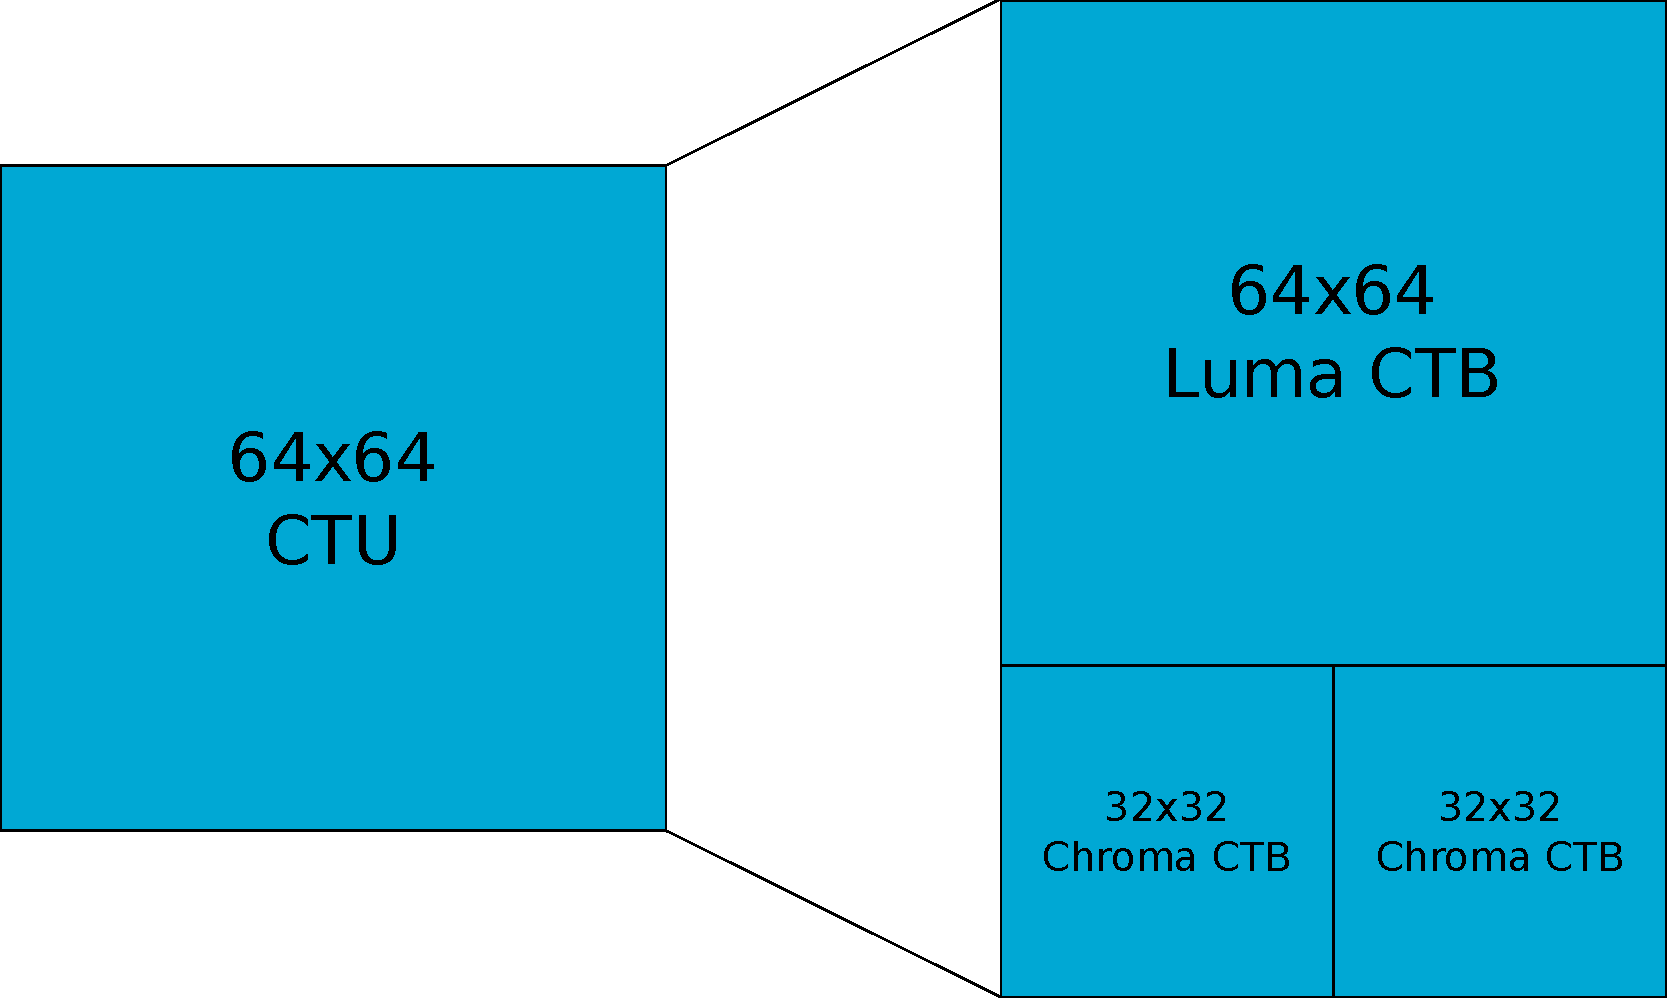
\includegraphics[scale=0.20]{Figures/CTU-CTB}
  \caption{Suddivisione del CTU in CTB}
\end{figure}
// Rivedere questo paragrafo: ovunque viene detto che il CTB è suddiviso \\
// in CU. \\
Il CTB può essere ulteriormente suddiviso in \emph{coding blocks} (CB), che 
sono il punto in cui viene decisa quale tipo di \emph{prediction} utilizzare.
Supponendo di avere un CTB di dimensione 64x64 la suddivisione può essere 
effettuata con CB grandi 64x64, 32x32, 16x16 o 8x8, ottenendo una struttura
detta \emph{quad-tree}, in cui il CTB è suddiviso ricorsivamente. 
Il CB, così come il CTB, consiste ancora nei tre blocchi Y, Cb e 
Cr, che definiscono un \emph{coding unit} (CU), ovverò l'unità in cui viene 
codificato il tipo di predizione. La scelta di quest'ultima è autonoma per ogni 
CU.
\begin{figure}[H]
  \centering
  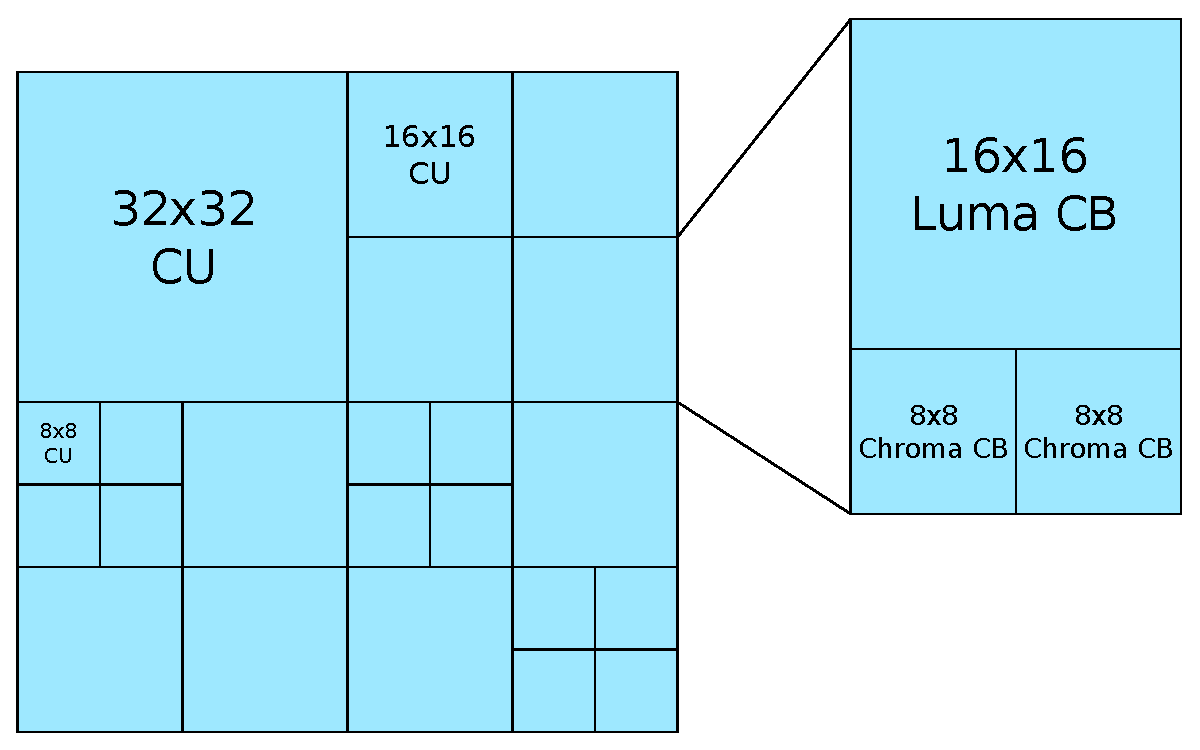
\includegraphics[scale=0.50]{Figures/CTB-CU-CB}
  \caption[Suddivisione del CTB in CU]{Suddivisione di un CTB 64x64 in una 
struttura a \emph{quadtree}}
\end{figure}
In caso ci sia bisogno di una maggiore precisione nella predizione (e.g., 
oggetti minuscoli che si muovono in un CB 8x8) è possibile suddividere i
\emph{coding block} in \emph{prediction block} (PB), che, in caso di 
\emph{inter prediction}, possono non seguire la struttura a \emph{quadtree} dei
blocchi precedenti:
\begin{figure}[H]
  \centering
  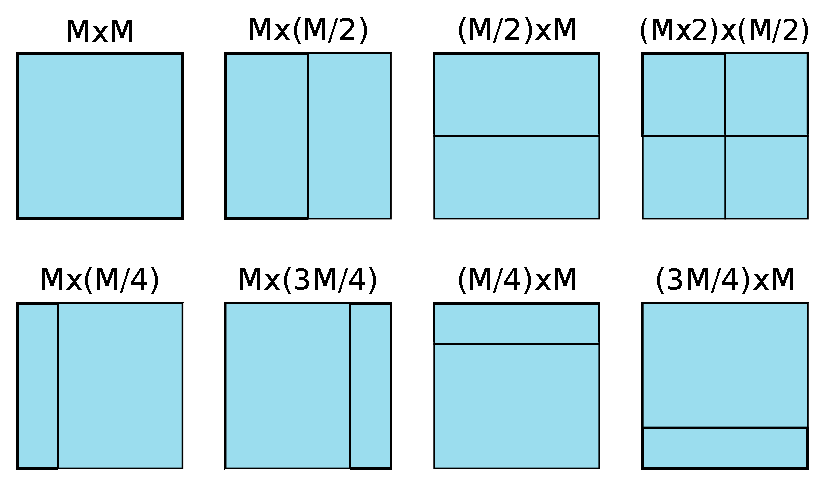
\includegraphics[scale=0.50]{Figures/PB}
  \caption{Possibili strutture di un \emph{prediction block}}
\end{figure}
Un PB definisce una regione che, per effettuare una predizione, utilizza gli 
stessi parametri di movimento: il numero di ipotesi di movimento (che può 
valere uno o due a seconda che si usi l'immagine precedente o quest'ultima 
e le successiva per cercare il blocco che si è mosso) e, per ognuna di queste, 
l'indice dell'immagine di riferimento e il vettore di movimento.
L'insieme dei tre PB, che possiedono lo stesso tipo di suddivisione, 
forma una \emph{prediction unit} (PU).
Per effettuare la codifica del segnale di errore un CB viene suddiviso in 
\emph{transform block}, dando forma ad una struttura a \emph{quadtree} che 
viene chiamata \emph{residual quadtree} (RQT); solitamente la suddivisione 
è mantenuta uguale per i TB Luma e Chroma.
%-------------------------------------------------------------------------------
%	SECTION 2
%-------------------------------------------------------------------------------
\section{Intra prediction}
Su un blocco di campioni contigui che possiedono gli stessi parametri 
predittivi, siano essi CB o PB, verrà eseguita la stessa 
\emph{intra prediction}.
Di quest'ultima esistono due tipologie a seconda delle caratteristiche 
del blocco: in caso di figure e strutture geometriche sarà utilizzata 
la \emph{angular prediction}, viceversa, se la predizione viene eseguita 
su contenuti meno strutturati, sarà eseguita una \emph{planar + DC prediction}. 
In entrambi i casi, la predizione si basa sui campioni contigui (o 
\emph{neighbour}) al blocco che si trovano a sinistra e a destra di 
quest'ultimo.

\paragraph*{Pre-filtering}
Prima di effettuare una delle due predizioni è possibile eseguire uno 
\emph{smoothing filter} sui campioni di riferimento, che dipende dal tipo di 
predizione che verrà successivamente eseguita. Le due possibilità sono le 
seguenti:
\begin{enumerate}
\item Un semplice \emph{lowpass filter} lineare con risposta all'impulso 
[1 2 1]/4 (a)
\item Se la dimensione del TB è 32x32 e i campioni di riferimento sono 
abbastanza ``morbidi'', questi vengono sostituiti con le corrispondenti 
interpolazioni lineari dei cambioni agli estremi (b)
\end{enumerate}

\begin{figure}[H]
  \centering
  \begin{tabular}{cc}
    \subfloat[]{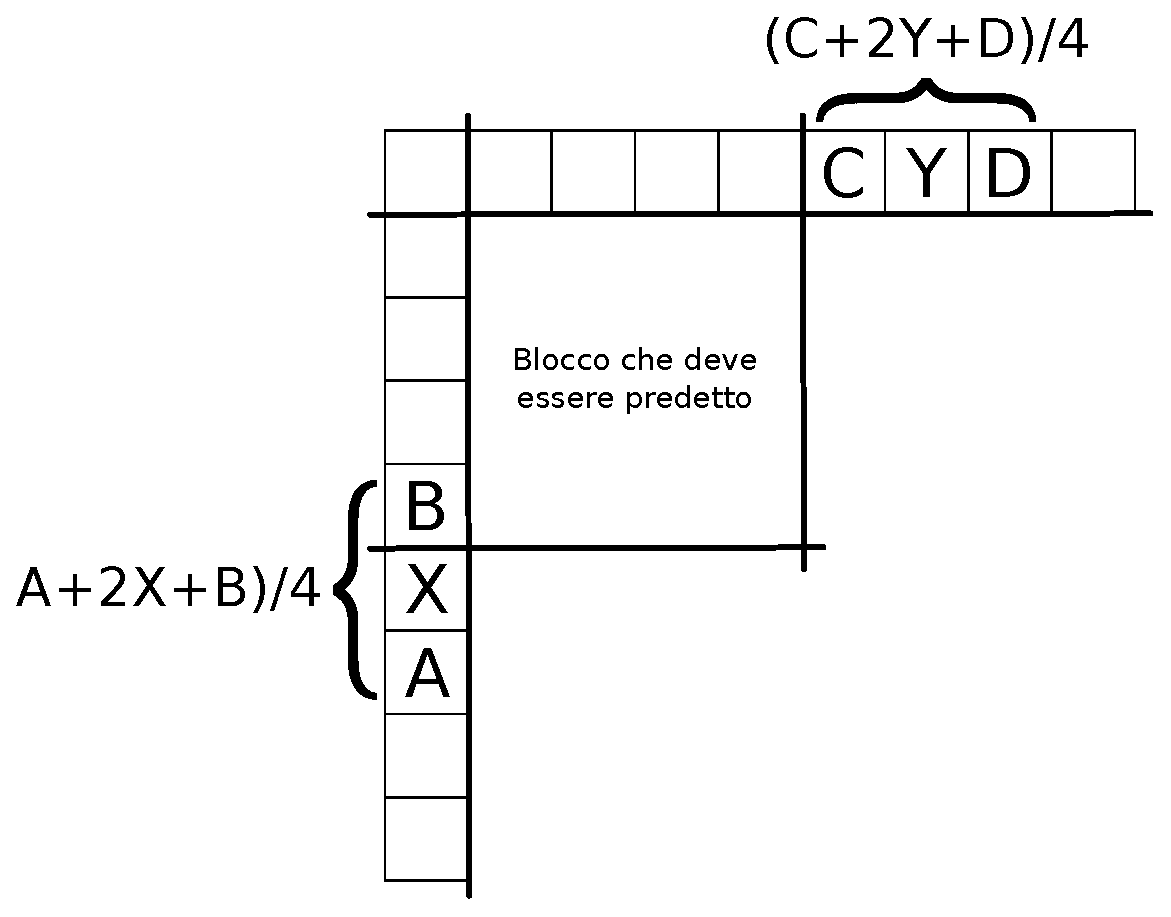
\includegraphics[scale=.35]{Figures/Filtering_a}}
    &
    \subfloat[]{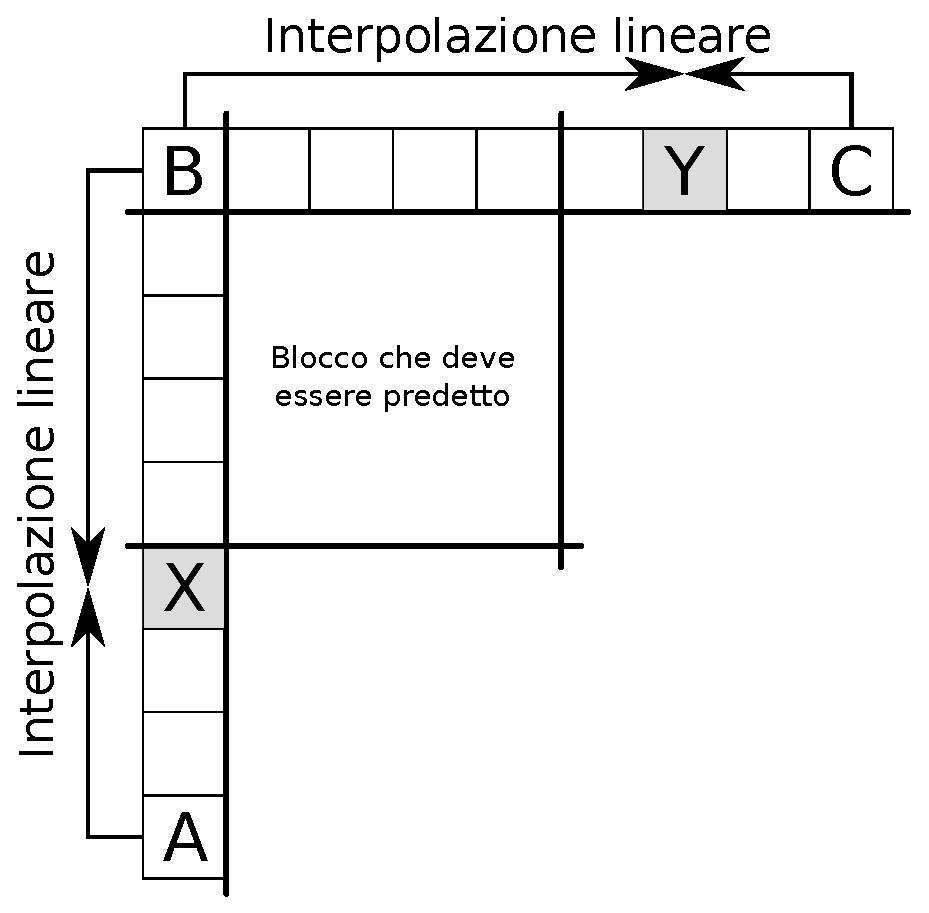
\includegraphics[scale=.35]{Figures/Filtering_b}}
  \end{tabular}
  \caption{I due diversi tipi di \emph{pre-filtering}}
\end{figure}
%-----------------------------------
%       SUBSECTION 1
%-----------------------------------

\subsection{Angular prediction}
Per la predizione angolare l'encoder deve scegliere uno tra 33 possibili angoli:
 questo tipo di predizione stima in modo accurato le strutture direzionali che 
sono tipicamente presenti nelle foto, tra cui le più frequenti risultano essere
 quelle orizzontali e verticali.
Per far fronte a quest'ultima circostanza, H.265 predispone gli angoli in modo 
che siano presenti in numero maggiore intorno alle due direzioni più frequenti;
 il numero totale di angoli e la loro disposizione è il risultato della ricerca 
di un buon \emph{trade-off} tra qualità e complessità computazionale 
dell'encoder.
\\
// Immagine qui
\\
Gli angoli prendono il nome di ``modi predittivi'' (\emph{prediction modes}) e 
il loro raggruppamento è diviso tra orizzontali e verticali.
Nell'immagine di cui sopra si può notare come gli angoli ``orizzontali'' siano 
quelli il cui segmento ha la sua origine in un campione collocato a sinistra, 
mentre l'origine del segmento degli angoli ``verticali'' risiede in un campione 
posizionato in alto.\\
Il parametro angolare $A$ indica la posizione, in termini di campioni, rispetto 
al campione centrale (che ha valore $0$).
Utilizzando il raggruppamento e il parametro $A$ è possibile identificare 
univocamente un modo predittivo; prendendo nuovamente in esame l'immagine la 
sigla $H+2$ corrisponde al modo predittivo 9, la sigla $H-2$ al modo predittivo 
11 e così via.\\
Per effettuare le predizioni dei campioni di un blocco viene prima costruito, 
per comodità, un array che contiene i campioni di riferimento riposizionati 
nell'ordine che risulta più conveniente per il modo predittivo scelto; infatti 
ogni campione $p[x][y]$ da predire viene ottenuto mediante l'interpolazione dei 
due campioni contigui all'interno dell'array di riferimento, con il fattore di 
interpolazione che risulta essere proporzionale all'angolo -o modo predittivo- 
selezionato.
%-----------------------------------
%       SUBSECTION 2
%-----------------------------------

\subsection{DC + Planar prediction }
\paragraph*{DC} La predizione DC prevede un valore costante per tutto il 
blocco, determinato dalla media dei valori dei campioni di riferimento che si 
trovano sopra e a sinistra del blocco.

\paragraph*{Planar} La predizione ``planare'' genera un blocco che presenta 
colori morbidi e privi di discontinuità marcate anche ai bordi. Questo è 
ottenuto tramite una semplice interpolazione, punto per punto, dei campioni di 
riferimento (evidenziati in giallo) con i loro estremi (evidenziati in grigio):
\begin{align*}
p[x][y] = 
%\left
[&\fcolorbox{yellow}{white}{$(N-1-x)*p(-1,y)$}+
  \fcolorbox{black!50}{white}{$(x+1)*p(N,-1)$}+\\
 &\fcolorbox{yellow}{white}{$(N-1-y)*p(x,-1)$}+
  \fcolorbox{black!50}{white}{$(y+1)*p(-1,N)$}+N] \gg log_2(N+1)
%\right]
\end{align*} 
dove $NxN$ è la dimensione del TB.
\\
// Inserire immagine
\\ 
L'immagine mostra come il risultato (c) sia la media di due interpolazioni: una 
orizzontale (a) e una verticale (b).
%-----------------------------------
%       SUBSECTION 3
%-----------------------------------

\subsection{Post-filtering}
Esistono tre casi in cui è necessario eseguire anche un filtraggio successivo, 
tipicamente quelli in cui si presentano brusche discontinuità ai bordi, e sono 
gli \emph{angular mode} esattamente orizzontali e verticali e la 
\emph{DC prediction}.
Il fatto che venga eseguito in sole tre evenienze è determinato dalla volontà 
di limitare la complessità computazionale di fronte a svantaggi che possono 
risultare  marginali, come nel caso delle predizioni diagonali, e dalla ricerca 
di un buon rapporto tra qualità e precedente complessità.
In seguito a test sperimentali è stato notato che le predizioni dei canali 
Chroma risultano sempre relativamente morbide; conseguentemente questo 
filtraggio viene eseguito solo sui canali Luma, e consiste nella modifica dei 
pixel ai bordi all'interno del blocco, secondo le seguenti modalità:
\begin{enumerate}
\item \emph{Angular prediction}, angolo verticale: \\
\begin{align*}
p(0,y)\mathrel{+}=\left(\frac{p*(-1,y)-p*(-1,-1)}{2}\right) 
\forall y \in {[0,N-1]}
\end{align*}

\item \emph{Angular prediction}, angolo orizzontale: \\
\begin{align*}
p(x,0)\mathrel{+}=\left(\frac{p*(x,-1)-p*(-1,-1)}{2}\right) 
\forall x \in {[0,N-1]}
\end{align*}

\item{ \emph{DC prediction}, posto $dcVal$ il valore della posizione: \\
\begin{align*}
p(0,0)=(p*(-1,0)+2dcVal+p*(0,-1)+2)*4
\end{align*}

Con i campioni ai bordi filtrati nel seguente modo:
\begin{align*}
p(x,0)&=(p*(x,-1)+3dcVal+2)*4 \forall y \in {[0,N-1]} \\
p(0,y)&=(p*(-1,y)+3dcVal+2)*4 \forall y \in {[0,N-1]}
\end{align*}

Dove $dcVal \in {[0,1]}$
}
\end{enumerate}

L'immagine seguente mostra un esempio di CTB Luma interamente predetto intra: \\

// Inserire immagine
%-------------------------------------------------------------------------------
%       SECTION 3
%-------------------------------------------------------------------------------

\section{Inter Prediction}
L'\emph{inter prediction} sfrutta la correlazione temporale dei frame per 
ottenere una \emph{motion compensated prediction} (MCP), ovvero un PB predetto 
a partire da PB ``predittori'' che appartegono a frame precedentemente 
decodificati, supponendo che nel PB predetto essi siano traslati: 
\\
// Inserire immagine
\\
Per ogni PB l'encoder ricava un vettore ${(\Delta x,\Delta y,\Delta t)}$ 
chiamato \emph{motion data}, dove ${(\Delta x,\Delta y)}$ è il 
\emph{motion vector} e indica la traslazione compiuta dal PB in questione, 
mentre ${(\Delta t)}$ è l'indice temporale dell'immagine a cui appartiene il PB 
predittore.
È anche possibile effettuare una ``bipredizione'': in questo caso si usano 
due \emph{motion data} ottenendo due MCP di cui viene ricavata la media (che 
può anche essere pesata) per ottenere il risultato, come illustra la figura 
precedente.
\\
Viene inoltre sfruttata la correlazione spaziale (ma sempre legata al tempo) 
dei \emph{motion vector}, basata sulla supposizione che i \emph{motion vector} 
relativi a PB spazialmente vicini non differiscano eccessivamente, eccezion 
fatta per eventuali punti di discontinuità come i cambi di oggetto. È inoltre 
ipotizzata una discreta continuità nel tempo per quanto riguarda i movimenti 
dell'intero \emph{frame}, escludendo variazioni brusche come i cambi di scena.
\\
Tutto questo viene tradotto nel concetto di \emph{motion vector predictor} 
(MVP); invece di trasmettere un \emph{motion vector} per ogni PB l'encoder 
trasmette l'errore o la \emph{motion vector difference} (MVD), tra quello 
predetto a partire da blocchi spazialmente o temporalmente contigui e quello 
normalmente calcolato con $MVD=MV-MP$.
Il decoder riceve la MVD e la sintassi necessaria a determinare il MVP (ovvero 
il tipo di predizione da utilizzare) e può dunque ricavare $MV$ come $MVD+MVP$.
 
Sebbene gli algoritmi che hanno preceduto H.265 (H.264, AVC) possiedano questo 
tipo di predizione, essi si limitano a calcolare $MVP$ come una media dei $MV$ 
vicini spazialmente: questa strategia non è più applicabile in HEVC a causa 
dell'elevata flessibilità delle strutture di predizione.
Il \emph{worst case scenario} presenta 16 $MV$ per lato da tenere in 
considerazione (come mostrato nell'immagine successiva), che porterebbe a 
complessità di codifica troppo elevate.

\begin{figure}[H]
  \captionsetup{justification=raggedright}
  \centering
  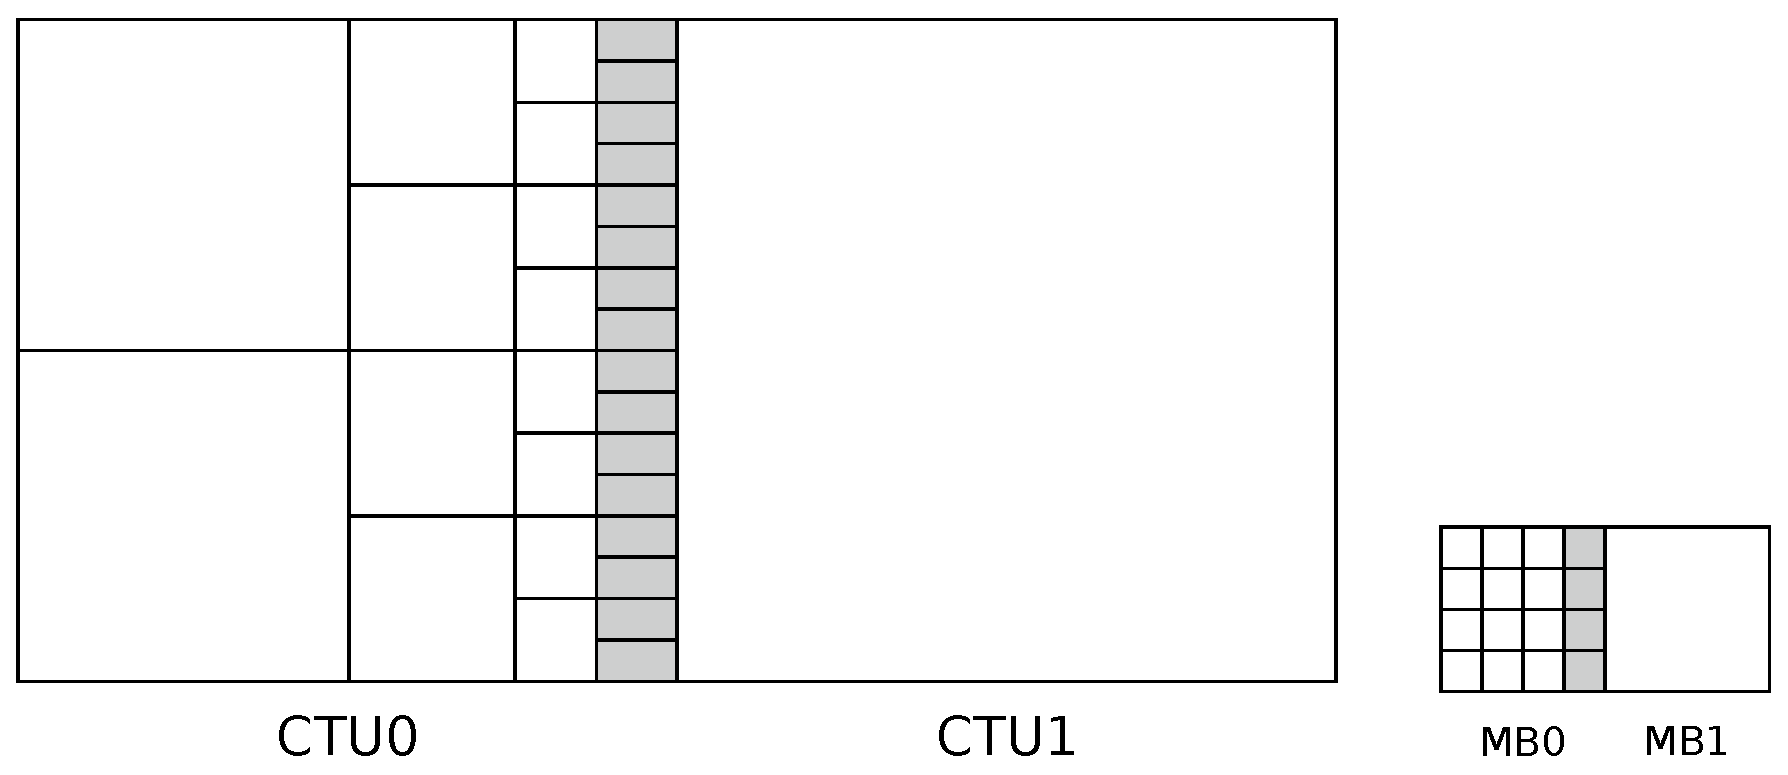
\includegraphics[scale=0.45]{Figures/Inter_pred_2}
    \caption[Numero massimo di \emph{motion vector} in H.265 e H.264]
    {Numero massimo di \emph{motion vector} in H.265 (a sinistra) e H.264 \\
      (a destra). CTU0 possiede 16 PB Luma 8x4 contigui a CTU1 che è composto da
      un solo PB Luma 64x64. MB0 (\emph{Macro Block)} contiene quattro 
      partizioni di predizione 4x4 affiancate a MB1 che consta di una 
      partizione 16x16. }
\end{figure}

H.265 mette a disposizione un algoritmo per la costruzione di vettori 
\emph{candidate MVP} chiamato \emph{advanced motion vector prediction} (AMVP), 
ottenuto in seguito ad esperimenti esaustivi volti a trovare oredizioni che 
minimizzassero la complessità di codifica pur mantenendo buoni livelli di 
predizione (i.e., bassa entropia del segnale di errore MVD).\\
Una parte della sintassi di HEVC serve a comunicare al decoder quale MVP 
utilizzare tra quelli candidati, che sono due e scelti nei modi seguenti:
\begin{itemize}
\item Due \emph{spatial candidate} che derivano da cinque blocchi spazialmente 
vicini;
\item Viene tenuto come riserva un \emph{temporal candidate} derivato da due 
blocchi co-locati e temporalmente vicini:
\begin{itemize}
\item Nel caso che i due \emph{spatial candidate} siano uguali, o se uno di loro
 non sia disponibile, i due vettori candidati saranno uno spaziale e uno 
temporale;

\item Se entrambi i candidati spaziali non fossero disponibili, verrà 
considerato il vettore candidato temporale di riserva ed uno 
\emph{zero motion vector};

\item Nell'eventualità che sia i candidati spaziali sia i candidati temporali 
non siano disponibili, entrambi i candidati saranno \emph{zero motion vector}.
\end{itemize}
\end{itemize}

Gli \emph{spatial candidate} sono ottenuti prendendo in considerazione cinque 
blocchi spazialmente vicini suddivisi in due gruppi: il gruppo A contenente i 
due blocchi in basso a sinistra rispetto a quello che si vuole predire, il 
gruppo B con al suo interno tre blocchi in alto.
Generalmente, se i vettori dei blocchi considerati sono ricondicibili allo 
stesso \emph{reference id} (l'indice dell'immagine a cui fanno 
riferimento) di quello del blocco che si vuole predire, tali vettori saranno 
MVP.
Viceversa, MVP sarà il vettore scalato secondo una formula che dipende dalla 
differenza temporale dei \emph{reference id}.
Non sono invece presi in considerazione blocchi a destra o in basso dal 
momento che tali PB non sono ancora stati decodificati e non sono disponibili 
al decoder per la predizione.
\\
Per quanto concerne il \emph{temporal candidate} si lavora su una immagine 
co-locata e temporalmente vicina della quale, in fase di decodifica, si 
possiedono tutte le informazioni (ovvero un frame già decodificato); diversi 
esperimenti hanno dimostrato che i blocchi da prendere in considerazione sono 
due: quello al centro e quello in basso a destra rispettivamente alla posizione 
del blocco che si vuole predire.
Specificamente il vettore viene predetto utilizzando sempre il blocco in basso 
a destra, salvo la mancanza di disponibilità d quest'ultimo; ciò significa che 
esso risiede fuori dai bordi dell'immagine o viola vincoli imposti per motivi 
di memoria.
\newline \\
Infine HEVC risolve un problema legato alla struttura di suddivisione delle 
immagini \emph{quadtree}: quest'ultime permettono una grande flessibilità 
delle dimensioni dei blocchi con un basso costo di \emph{overhead} in termini 
di \emph{bit rate}. Per l'\emph{inter prediction} la struttura a \emph{quadtree}
 permette di suddividere minuziosamente quelle parti di immagine dhe presentano 
bruschi movimenti rispetto alle parti più statiche che non richiedono una 
grande informazione di movimento. Questo tipo di raggruppamento, tuttavia, 
origina facilmente bordi ineffettivi (\emph{over segmentation}); HEVC dispone 
di un  algoritmo di \emph{block merging} che consente di raggruppare PB con 
uguali parametri di predizione in modo da trasmetterne una sola copia.
\\
Nell'esempio mostrato dall'immagine seguente la parte a) è l'immagine 
originale, b) è l'immagine scomposta in PB secondo la struttura a 
\emph{quadtree} mentre c) mostra il risultato del \emph{block merging}.
\\
// Inserire immagine 
\\
%-------------------------------------------------------------------------------
%       SECTION 4
%-------------------------------------------------------------------------------

\section{Transform and Quantization}
Nel \emph{block-based video coding} i segnali di errore residui che derivano 
dalle predizioni intra o inter vengono trasformati e quantizzati prima di 
essere trasmessi.
Più nel dettaglio, un'immagine è suddivisa in blocchi quadrati di dimensione $NxN$, dove $N=2^M$ con $M \in \mathbb{N}$. Per ogni blocco esisterà un blocco 
residuo $U$ che verrà trasformato e quantizzato. \\
L'immagine mostra il percorso dei dati durante la fase di encoding (a) e 
di decoding (b):
\begin{figure}[H]
  \centering
  \begin{tabular}{cc}
    \subfloat[]{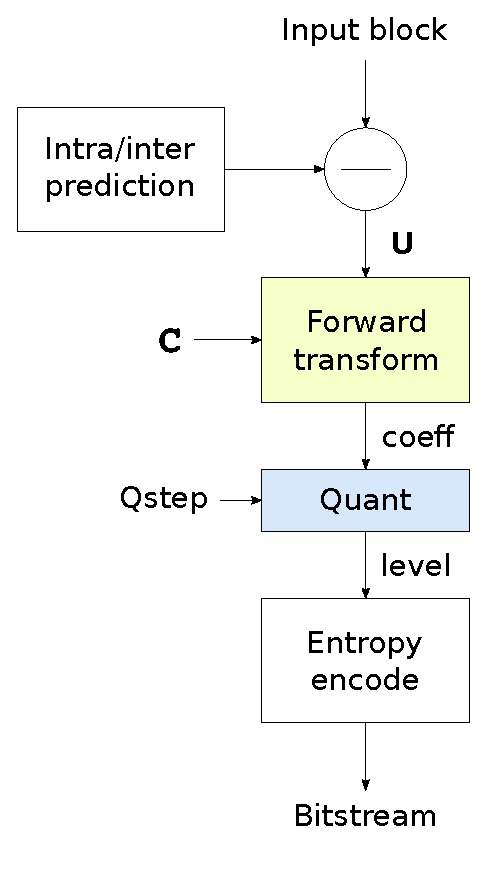
\includegraphics[scale=.66]{Figures/Transf_and_quant_a}}
    &\qquad
    \subfloat[]{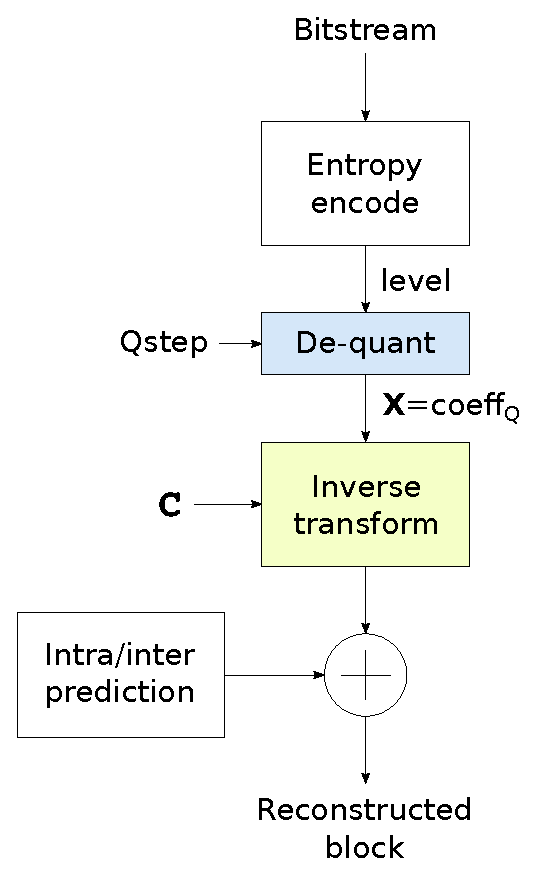
\includegraphics[scale=.66]{Figures/Transf_and_quant_b}}
  \end{tabular}
  \caption{\emph{Data flow} di encoding e decoding.}
\end{figure}
\subsection{Transform}
Tipicamente le trasformate sono delle matrici costruite in modo tale che, in 
assenza di quantizzazione, sommando trasformata e trasformata inversa si 
ottenga un risultato praticamente lossless.
HEVC utilizza due tipologie di trasformate, ovvero quelle derivate dalla DCT e
quelle derivate dalla DST; fornisce inoltre delle matrici precostruite per 
eseguire l'antitrasformata DCT e DST per tutte le possibili dimensioni dei 
blocchi: $4x4$, $8x8$, $16x16$ e $32x32$.
Queste matrici contengono approssimazioni ad interi con precisione finita dei 
coefficienti di trasformazione DCT-II; questo sistema riduce di molto la 
complessità di encoder e decoder, e risolve un problema che era presente in 
H.261, ovvero la deriva dovuta a lievi disallineamenti nella rappresentazione 
fixed point dei coefficienti tra la matrice di trasformazione, costruita 
arbitrariamente dal'implementatore dell'encoder, e quella di antitrasformazione 
fornita dallo standard. \\
Errori di questo tipo si ripercuotono amplificati in ogni immagine successiva, 
costringendo a dover trovare un modo di ovviare al problema (il sopracitato 
H.261 costringeva un aggiornamento periodico del segnale che consisteva in una 
immagine codificata interamente intra).
\subsection{Quantization}
Con ``quantizzazione'' si intende la divisione dei valori trasformati 
utilizzando un passo di quantizzazione $Q_s$ (\emph{quantization step}) definito
 attraverso il parametro di quantizzazione $Q_p$ come segue:
\begin{align*}
Q_s = \left(2^{\frac{1}{6}}\right)^{(Q_p-4)}
\end{align*}
Dalla formula si può notare come una variazione di $1$ per $Q_p$ si traduca in 
una moltiplicazione di $Q_s$ per un fattore $2^{\frac{1}{6}}\approx 1.12$, ovvero 
nell'incremento di $Q_s$ del $12\%$. Una variazione di $6$ si traduce in un 
raddoppiamento di $Q_s$ \\
Si può anche eseguire una quantizzazione \emph{frequency dependent} specificando
 una matrice $w$ con un valore di quantizzazione per ogni frequenza, con un 
risultato che risulta il seguente:
\begin{align*}
q[x][y] = \frac{tc[x][y]}{q[x][y]*Q_s}+offset
\end{align*}
dove $tc$ sono i coefficienti trasformati. \\
Si ottiene una compressione in quanto i valori, una volta quantizzati, verranno 
arrotondati all'intero più vicino. Il fine è quello di portare a 0 il maggior 
numero possibile di coefficienti in modo che la codifica successiva (marcata 
come \emph{Entropy encode}) sia in grado di comprimere al meglio la sequenza in 
uscita; dividendo un intero per un numero più grande il risultato sarà più 
vicino a zero. Tipicamente le matrici di quantizzazione possiedono valori più 
grandi alle basse frequenze e viceversa alle alte, perché il contenuto utile 
per il sistema visivo umano è concentrato alle basse frequenze.

%-------------------------------------------------------------------------------
%       SECTION 5
%-------------------------------------------------------------------------------

\section{In-Loop Filters}
Lo standard ibrido di codifica HEVC scompone i frame attraverso una struttura a 
blocchi per effettuare la compressione; questa suddivisione porta spesso alla 
comparsa di artefatti che danno alle sequenze video un'aspetto quadrettato, 
peggiorandone la qualità visiva. Un esempio tipico di causa della discontinuità 
tra i blocchi è la predizione inter di due blocchi contigui che nel frame
 di riferimento erano distanti, oppure anche la codifica di due blocchi contigui
 con modalità predittive differenti (due intra diversi, una inter e una intra, 
etc.). Per porre rimedio a questi artefatti lo standard HEVC specifica due 
filtraggi: il \emph{deblocking filter} e il \emph{sample adaptive offset} (SAO).
\\ \\
Questi filtraggi sono chiamati \emph{in-loop filters} perché vengono eseguiti 
all'interno dei cicli di encoding/decoding, e i risultati vengono utilizzati 
nei cicli successivi oltre che durante la visualizzazione delle sequenze 
decodificate; in questo modo si trae vantaggio da questa procedura anche durante
 il decoding dei frame successivi, preché le predizioni inter vengono effettuate
 a valle di frame reference di maggiore qualità.
\\ \\
Il \emph{deblocking filter} si occupa di smussare i confini tra due blocchi in 
cui è presente una discontinuità, cercando di lavorare solo su quelle 
introdotte durante la compressione e non quelle originariamente presenti nella 
sequenza. \\
Il SAO, invece, si occupa di ridurre gli artefatti dovuti a trasformazioni e 
quantizzazioni grossolane (chiamati \emph{ringing artifacts}), ed opera 
sull'output del \emph{deblocking filter} in cascata. \\
Visto che i due filtraggi operano su due artefatti diversi, i loro benefici 
sono additivi se eseguiti insieme.
\subsection{Deblocking Filter}
Il \emph{deblocking filter} si applica solo ai confini tra blocchi di tipo CU, 
PU o TU e non al loro interno; durante la codifica  l'encoder considera gruppi 
di quattro vettori di campioni perpendicolari ai confini dei blocchi. 
Specificamente l'encoder esegue alcuni controlli sul primo e sul quarto vettore 
per decidere:
\begin{itemize}
\item Se eseguire il filtraggio o meno;
\item In caso positivo quale filtraggio applicare tra \textbf{normal} e 
\textbf{strong}.
\end{itemize}
Questi semplici controlli misurano un indice di distorsione dei vettori di 
campioni rispetto ad una delle funzioni continue più semplici, ovvero una rampa 
che attraversa il confine \textbf{/*(di che cosa?)*/}. Se questo indice supera 
una certa soglia, che dipende dal passo di quantizzazione $Q_p$ secondo una 
\emph{look-up table}, si esegue il filtraggio.

\begin{figure}[H]
  \captionsetup{justification=raggedright}
  \centering
  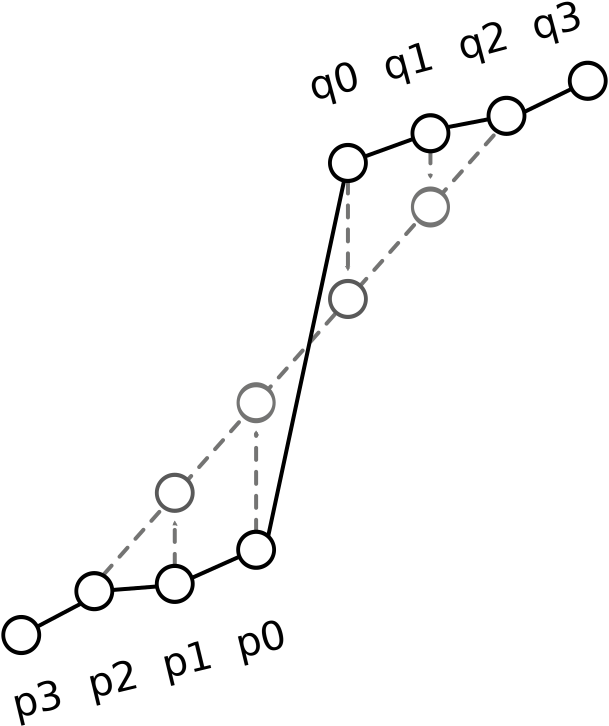
\includegraphics[scale=0.45]{Figures/Deblocking_filter}
    \caption[Filtraggio \emph{deblocking} di tipo \textbf{normal}]
    {Filtraggio \emph{deblocking} di tipo \textbf{normal}: la linea nera mostra
      il confine originale del blocco, la linea grigia tratteggiata quello 
      nuovo}
\end{figure}

L'immagine mostra il risultato di un filtraggio \textbf{normal} eseguito su un 
vettore di 8 campioni, con questi ultimi appartenenti a due blocchi confinanti 
chiamati $P$ e $Q$. \\
In generale, un filtraggio \textbf{normal} può arrivare a modificare fino a due
campioni per lato avvicinandoli alla rampa, come accade nell'immagine.
Il filtraggio \textbf{strong} viene utilizzato nelle aree che racchiudono 
contenuti a bassa frequenza, ovverosia quelle in cui il sistema visivo umano è 
più sensibile alle discontinuità, e consiste in un filtraggio lineare lowpass 
che comprende tre campioni per lato.
\\ \\
Il filtraggio \emph{deblocking} descritto interessa solamente il canale luma, 
dal momento che per i canali chroma si opera un filtraggio analogo ma più 
grossolano, in cui vengono eseguiti molti meno controlli e vengono considerati 
meno campioni: ciò permette di ridurre la complessità dell'encoder a fronte di 
una bassa perdita di qualità, sempre considerando il fatto che i canali chroma 
sono meno importanti per il sistema visivo umano.
\subsection{Sample Adaptive Offset - SAO}
 
% Chapter Template

\chapter{La piattaforma ARM embedded} % Main chapter title

\label{Chapter5} % Change X to a consecutive number; for referencing this chapter elsewhere, use \ref{ChapterX}

\lhead{Capitolo 5. \emph{La piattaforma ARM embedded}} % Change X to a consecutive number; this is for the header on each page - perhaps a shortened title

%----------------------------------------------------------------------------------------
%	SECTION 1
%----------------------------------------------------------------------------------------

\section{Sistema \emph{embedded}}

%Sistema embedded: che cos'è, a che cosa serve, chi rientra nella categoria?
%Differenza tra special purpose e general purpose, importanza dell'applicazione
// Rivedere questo incipit \\
Un sistema può essere visto come un insieme di più parti che collaborano al fine
di svolgere un determinato compito; considerando gli  ambiti informatici ed 
elettronici un sistema \emph{embedded} (tradotto solitamente con ``sistema 
integrato'') 

%----------------------------------------------------------------------------------------
%	SECTION 2
%----------------------------------------------------------------------------------------

\section{Processori ARM}

%-----------------------------------
%       SUBSECTION 1
%-----------------------------------

\subsection{Il processore AllWinner A20}

%----------------------------------------------------------------------------------------
%       SECTION 3
%----------------------------------------------------------------------------------------

\section{Il \emph{single-board} computer Banana Pi M1}
\begin{center}
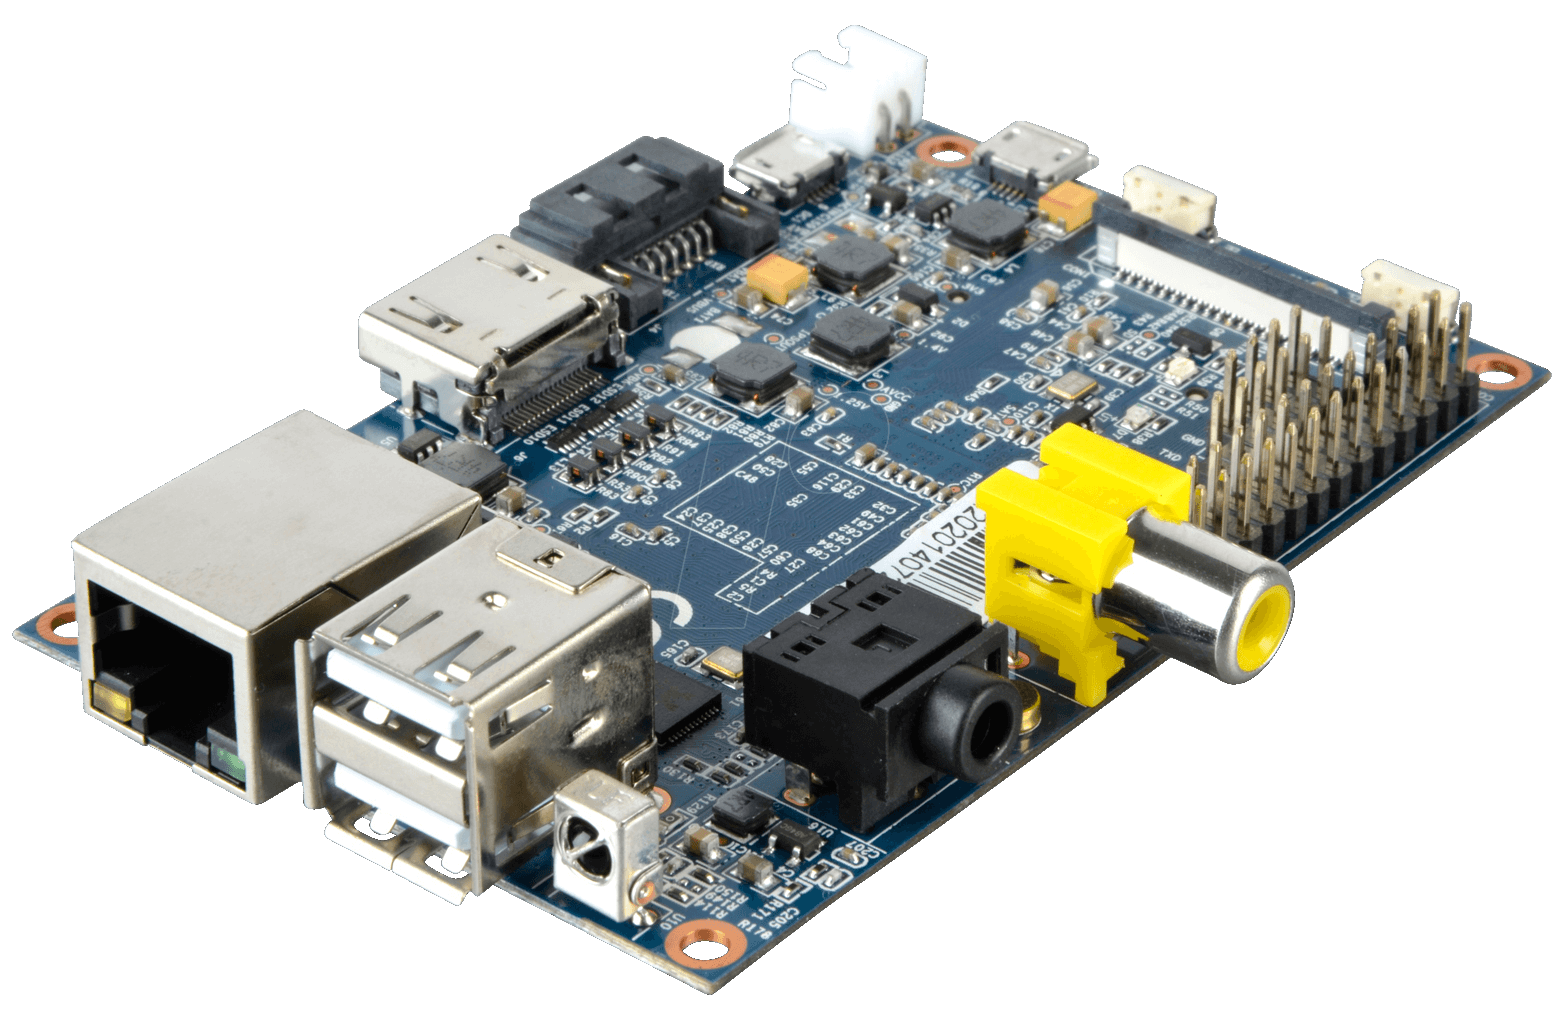
\includegraphics[scale=0.175]{Figures/bananapi.png}\\[0.5cm]
\end{center} 
% Chapter 

\chapter{Il progetto} % Main chapter title

\label{Chapter6} % Change X to a consecutive number; for referencing this chapter elsewhere, use \ref{ChapterX}

\lhead{Capitolo 6. \emph{Il progetto}} % Change X to a consecutive number; this is for the header on each page - perhaps a shortened title

%-------------------------------------------------------------------------------
%	SECTION 1
%-------------------------------------------------------------------------------

\section{Il setup della piattaforma}
La prima decisione che ha riguardato la piattaforma è stato il sistema 
operativo da installare. Vi sono a disposizione diversi sistemi 
Unix-like\footnote{http://www.lemaker.org/portal.php?mod=list\&catid=4}, 
dai più personalizzabili (come Gentoo o Arch Linux) a quelli più
 \emph{user-friendly} (come Lubuntu); la nostra scelta è ricaduta su Bananian, 
una distribuzione che deriva da Debian 7, appositamente ottimizzata per il 
Banana Pi, che abbiamo ritenuto essere il giusto compromesso tra usabilità
e assenza di software preinstallato a noi non necessario. \\
Nonostante la possibilità di lavorare senza ambiente grafico, da terminale, 
risparmiando qualche decina di \emph{megabyte} di RAM, inizialmente abbiamo 
deciso di avvalerci di LXDE, un ambiente desktop estremamente leggero, in modo da 
velocizzare la maggior parte delle nostre interazioni con il sistema. \\
\\ \\
Essendo tre persone a lavorare su una sola piattaforma, abbiamo optato 
per collocare la \emph{board} in un laboratorio dell'università, dotandola
di un sistema di controllo remoto basato su \emph{virtual network computing} 
(VNC), un sistema che utilizza un protocollo \emph{remote framebuffer} (RBF) 
per l'accesso remoto alle interfacce grafiche utente (meglio conosciute come 
\textbf{GUI}s, \textbf{G}raphical \textbf{U}ser \textbf{I}nterfaces). Inoltre, 
per facilitare l'accesso ai dati presenti sulle periferiche di memorizzazione, 
abbiamo dotato il Banana Pi di un server \emph{file transfer protocol} (FTP).
\\ \\ 
Tuttavia, nella fase finale del progetto, l'intefaccia grafica è stata 
abbandonata in modo da permettere una risposta del sistema più immediata e una 
minore allocazione di risorse; è stato dunque possibile disattivare 
l'accelerazione hardware, necessaria in un ambiente grafico, permettendo il 
risparmio di circa 30MB di RAM. Insieme alla GUI è stata accantonato il 
controllo remoto tramite VNC (fortemente dispendioso a causa del suo approccio 
\emph{pixel-based}) a favore di un accesso tramite SSH (\emph{secure shell}), 
più essenziale e meno dispersivo.

%-------------------------------------------------------------------------------
%	SECTION 2
%-------------------------------------------------------------------------------

\section{I tool per la compilazione}

%-----------------------------------
%       SUBSECTION 1
%-----------------------------------

\subsection{Il compilatore GCC}

%-----------------------------------
%       SUBSECTION 2
%-----------------------------------

\subsection{Il tool make}

%-------------------------------------------------------------------------------
%	SECTION 3
%-------------------------------------------------------------------------------

\section{I tool per valutare le prestazioni}
Per la valutazione delle prestazioni degli encoder da ottimizzare, è stato 
fatto uso di due strumenti software:
\begin{itemize}
\item Valgrind
\item gperftools
\end{itemize}
Entrambi \emph{opensource}, offrono diversi strumenti per l'analisi dinamica 
di un software; quelli utilizzati in questo progetto sono stati
\emph{Cachegrind} e \emph{Callgrind} per quanto riguarda il primo e il 
\emph{CPU profiler} del secondo.
%-------------------------------------------------------------------------------
%	SECTION 3
%-------------------------------------------------------------------------------

\section{I software di encoding presi in considerazione}
Inizialmente, tre software di encoding sono stati individuati come possibili
candidati per il progetto:
\begin{itemize}
\item f265
\item HM (\textbf{H}EVC Test \textbf{M}odel)
\item x265
\end{itemize}
Il primo è stato subito scartato non appena è stato chiaro che il sorgente non 
è compatibile con la piattaforma in nostro possesso (il codice è stato scritto 
unicamente per architettura x86).
I rimanenti due sono stati oggetto di 
%-------------------------------------------------------------------------------
%	SECTION 4
%-------------------------------------------------------------------------------

\section{Test preliminari}

%-------------------------------------------------------------------------------
%	SECTION 5
%-------------------------------------------------------------------------------

\section{Individuazione dei moduli H.265}

%-----------------------------------
%       SUBSECTION 1
%-----------------------------------

\subsection{Il tool KCacheGrind / QCacheGrind}

%-------------------------------------------------------------------------------
%	SECTION 6
%-------------------------------------------------------------------------------

\section{Strategie di ottimizzazione}

%-----------------------------------
%       SUBSECTION 1
%-----------------------------------

\subsection{Compilation flags}
Per prima cosa abbiamo dedicato del tempo allo studio delle opzioni di 
compilazione fornite da GCC (\emph{GNU Compiler Collection}) al fine di partire 
da una ``base stabile" da ottimizzare.\\
Particolare attenzione è stata dedicata ai \emph{flag} dedicati al 
miglioramento delle performance ed a quelli specifici per ARM.\\
\\
Senza alcuna opzione di compilazione espressa l'obiettivo del compilatore è 
quello di ridurre il più possibile il costo della compilazione e di rendere al 
contempo praticabile il \emph{debug} del programma. Per rendere possibile il 
//debug ciò è necessario in primo luogo che ogni \emph{statement} sia 
indipendente: è possibile fermare l'esecuzione in qualsiasi punto utilizzando 
un \emph{breakpoint} al fine di assegnare a piacere valori alle variabili e/o 
di modificare il \emph{program counter}, ottenendo i risultati attesi dal 
codice.\\
\\
Il compilatore ottimizza il codice basandosi sulla conoscenza che ha del 
programma. Non tutte le ottimizzazioni sono controllabili direttamente via 
\emph{flag}.\\
\\
Passiamo ora ad una breve descrizione delle opzioni utilizzate e dei loro 
effetti sull'eseguibile generato.

Famiglia `-O': opzioni dedicate all'ottimizzazione delle performance e/o della 
dimensione del compilato. La `O' è un diminutivo di ``Optimize".\\
Si distinguono vari livelli di ottimizzazione messi a disposizione dal 
compilatore GCC:
\begin{itemize}
\item \verb|-O0|\\
Opzione predefinita: riduce il tempo di compilazione cercando di dare la 
migliore esperienza di \emph{debug} possibile.
\item \verb|-O / -O1|\\
Abilita tutte le opzioni specificate da \verb|-O0|.\\
Il compilatore cerca di ridurre la dimensione del compilato ed il tempo di 
esecuzione utilizzando \emph{flag} che non peggiorano drasticamente il tempo 
di compilazione.
\item \verb|-O2|\\
Abilita tutte le opzioni specificate da \verb|-O / -O1|.\\
Vengono eseguite tutte le ottimizzazioni che non coinvolgono un 
\emph{trade-off} spazio-velocità. Rispetto al precedente migliora le 
prestazioni allungando il tempo di compilazione.
\item \verb|-Os|\\
Abilita tutte le opzioni specificate da \verb|-O2| che tipicamente non 
aumentano la dimensione dell'eseguibile. Vengono eseguite tutte le 
ottimizzazioni a favore dello spazio occupato dal compilato. La `s' è un 
diminutivo di ``size".
\item \verb|-O3|\\
Abilita tutte le opzioni specificate da \verb|-O2|.\\
Vengono eseguite tutte le ottimizzazioni a favore della velocità di esecuzione. 
Il tempo di compilazione aumenta così come lo spazio occupato dall'eseguibile 
generato. E' il massimo livello di ottimizzazione possibile insieme ad 
\verb|-Ofast|.
\item \verb|-Ofast|\\
Abilita tutte le opzioni specificate da \verb|-O3|.\\
Ignora l'adesione rigorosa allo standard abilitando \verb|-ffast-math|.
\item \verb|-Og|\\
Ottimizza l'esperienza di \emph{debug} abilitando tutte le opzioni che non 
interferiscono con quest'ultimo.
\end{itemize}

Opzioni di ottimizzazione indipendenti dall'hardware:

\begin{itemize}
\item \verb|-ftree-vectorize|\\
Abilita la vettorizzazione dei \emph{tree}.
// Che cos'è un tree?\\
Il compilatore cerca di riorganizzare dati in vettori permettendo così 
l'utilizzo di istruzioni SIMD (\emph{Single Instruction Multiple Data}) al fine 
di migliorare il tempo di esecuzione del codice.\\
Essa abilita inoltre \verb|-ftree-loop-vectorize| e 
\verb|-ftree-slp-vectorize|, che abilitano rispettivamente la vettorizzazione 
dei \emph{loop} e dei \emph{basic block}.
\item \verb|-finline-functions|\\
Considera tutte le funzioni come candidate per un possibile \emph{inlining}, 
anche quelle che non sono dichiarate esplicitamente come \verb|inline|.\\
Il compilatore decide attraverso un calcolo euristico di effettuare o no 
l'\emph{inlining} della funzione. 
\item \verb|-funswitch-loops|\\
Abilitata automaticamente con l'opzione \verb|-O3|.\\
Sposta i \emph{branch} con condizioni che non dipendono dal \emph{loop} al di 
fuori di quest'ultimo, duplicandolo su entrambi i \emph{branch} e modificandolo 
tenendo conto del risultato della condizione.
\item \verb|-funroll-loops|\\
Abilita l'\emph{unrolling} dei \emph{loop} per i quali è possibile determinare 
il numero di iterazioni a \emph{compile time}.
// Aggiungere -fwhole-program?
\end{itemize}

Opzioni di ottimizzazione specifiche per l'hardware ARM:

\begin{itemize}
\item \verb|-march=|\emph{name}\\
Specifica il nome dell'architettura ARM di destinazione.\\
Questo parametro viene utilizzato da GCC per determinare che tipo di istruzioni 
possono essere emesse quando viene generato il codice assembly relativo al 
programma.
\item \verb|-mtune=|\emph{name}\\
Specifica il nome del processore ARM per il quale GCC deve ottimizzare il 
codice. Su alcune implementazioni possono essere ricavate prestazioni migliori 
specificando questa opzione.
\item \verb|-mfpu=|\emph{name}\\
Specifica quale hardware (o emulazione hardware) \emph{floating-point} è 
disponibile sul dispositivo.\\
Quest'opzione è \underline{necessaria} per poter utilizzare le varie SIMD (in 
questo caso NEON) messe a disposizione dall'architettura ARM.
\item \verb|-mfloat-abi=|\emph{name}\\
Specifica quale ABI (o \emph{Application Binary Interface}) utilizzare per le 
operazioni \emph{floating-point}. // Che cos'è un ABI? \\
Quest'opzione è \underline{necessaria} per poter utilizzare le varie SIMD (in 
questo caso NEON) messe a disposizione dall'architettura ARM.
\end{itemize}

Opzioni del linguaggio e del \emph{debug}.

\begin{itemize}
\item \verb|-fopt-info-|\emph{options}\\
Mostra un \emph{log} contenente informazioni su ciò che è o non è stato 
ottimizzato.
\item \verb|-std=|\emph{name}\\
Determina quale standard utilizzare per il linguaggio C da compilare.
\item \verb|-pthread|\\
Abilita il supporto al \emph{multithreading} con la libreria \emph{phtreads}.
\end{itemize}

Queste opzioni sono state testate modificando il file \verb|makefile.base|, 
contenuto nella cartella \verb|/build/linux/common/|. Di seguito le linee 
dall'originale:\\

\begin{lstlisting}[language=make]
# default cpp flags for all configurations
CPPFLAGS          = -fPIC $(DEFS) -I$(CURDIR)/$(INC_DIR) $(USER_INC_DIRS) -Wall
                    -Wshadow -Wno-sign-compare -Werror
# debug cpp flags
DEBUG_CPPFLAGS    = -g -D_DEBUG
# release cpp
RELEASE_CPPFLAGS  = -O3 -Wuninitialized
\end{lstlisting}

Per prima cosa è stato cambiato il livello di ottimizzazione da \verb|-O3| a 
\verb|-Ofast| per quanto riguarda i \verb|RELEASE_CPPFLAGS|.\\
Questa modifica è stata effettuata al fine di migliorare le \emph{performance} 
sulle operazioni matematiche, è stato inoltre verificato che il comportamento 
del programma non fosse cambiato (\verb|-ffast-math| può portare a risultati 
sbagliati in certe configurazioni).\\
Assieme a suddetta modifica è stato cambiato il \emph{flag} \verb|-g| in 
\verb|-Og| per quanto riguarda i \verb|DEBUG_CPPFLAGS|.\\
Questo al fine di velocizzare il più possibile il \emph{debug} 
dell'applicazione, particolarmente lento utilizzando \verb|-g|.\\
Sono state poi inserite tutte le opzioni relative all'hardware ARM in 
\verb|CPPFLAGS|, i \emph{flag} condivisi da tutte le configurazioni.\\
Nello specifico sono state inserite le seguenti voci: \verb|-march=armv7-a|, 
\verb|-mtune=cortex-a7|, \verb|-mfpu=neon|, \verb|-mfloat-abi=softfp|.\\
Subito dopo questa modifica è stato ancora aggiunta ai \verb|RELEASE_CPPFLAGS| 
l'opzione \verb|-ftree-vectorize|.\\
\\
Prima di iniziare la modifica vera e propria del codice è stata effettuata 
un'analisi mediante l'utilizzo di \verb|-fopt-info-vec-optimized| al fine di 
sapere cosa fosse stato già vettorizzato automaticamente da GCC. Questo ci ha 
permesso di focalizzarci maggiormente sulle funzioni onerose non modificate.\\
\\
E' stato inoltre deciso di rendere \emph{multithread} il programma.\\
E' stato in primo luogo provato il \emph{multithreading} offerto dallo standard 
C++11, aggiungendo quindi \verb|-std=c++11| alle opzioni esistenti.\\
Avendo però notato un degrado delle performance generali in \emph{single 
thread}, sì è deciso di utilizzare la libreria \emph{pthreads} e quindi di 
sostituire il \emph{flag} \verb|-std=c++11| con \verb|-pthread|.

Il file \verb|makefile.base| finale è quindi il seguente:\\

\begin{lstlisting}[language=make]
# default cpp flags for all configurations
CPPFLAGS          = -fPIC $(DEFS) -I$(CURDIR)/$(INC_DIR) $(USER_INC_DIRS) -Wall 
                    -Wshadow -Wno-sign-compare -Werror -march=armv7-a 
                    -mtune=cortex-a7 -mfpu=neon -mfloat-abi=softfp -pthread
# debug cpp flags
DEBUG_CPPFLAGS    = -Og -D_DEBUG
# release cpp
RELEASE_CPPFLAGS  = -Ofast -Wuninitialized -ftree-vectorize
\end{lstlisting}


// Tentativi con -fwhole-program.\\
// gcc-4.7 non vettorizzava ARM, gcc-4.9 sì.\\
// Risultati\\
%-----------------------------------
%       SUBSECTION 2
%-----------------------------------

\subsection{Assembly}
// IMPOSTA FONT CONSOLAS PER I LISTATI \newline
// INGRANDISCI IL FONT DI TESTO E LISTATI \newline
Un'altra ottimizzazione sperimentata inizialmente è stata
 la stesura di funzioni in Assembly nel tentativo di ottimizzare alcune parti 
 di codice delle funzioni più onerose di HM.
Le principali caratteristiche del linguaggio Assembly ARM che velocizzano un 
programma sono le istruzioni condizionali e il \emph{barrel
 	 shifter}. \newline
Le istruzioni condizionali sono normali istruzioni la cui esecuzione dipende
dal valore di determinati \emph{flag}. In questo modo è possibile evitare
parecchi branch condizionali che rallentano il codice perché rompono la
\emph{pipeline}.\newline
Il \emph{barrel shifter} è un'unità che compie una pre-elaborazione di uno dei 
due operandi di un'istruzione attraverso una normale operazione di shift dei 
bit. \newline
//SPIGA PERCHE IL BARREL SHIFTER VELOCIZZA (NON AGGIUNGE TEMPO ESECUZIONE)
//AGGIUNGI IMMAGINE BARREL SHIFTER \newline

\par Per esempio, la funzione matematica $\text{clamp}(x) = 
\max(a,\min(x,b))$, assente dalla libreria standard, viene implementata da 
\verb+filter+ in questo modo:
\lstinputlisting[language=C,caption=]{Codes/cclamp.c}
Questo codice viene tradotto in \verb|-Ofast| in una dozzina di istruzioni con 
due \emph{compare}. Notando che nel codice di HM \verb|minVal| vale sempre 0, è 
possibile introdurre un'ottimizzazione che sfrutta il barrel shifter. \newline
Segue il confronto tra l'estratto del codice Assembly generato da GCC (a 
sinistra) e quello da noi scritto per eseguire clamp.
// ALLINEA VERTICALMENTE I DUE LISTATI

\lstset{style=cstyle}
\begin{center}
  \begin{tabularx}{\textwidth}{ X | c }
  	\hline
    \lstinputlisting[caption=]{Codes/armgccclamp.s}
    \xdef\tempwidth{\thelstlisting\linewidth} &
    \lstinputlisting[stepnumber=0,caption=]{Codes/armclamp.s} \\
    \hline
  \end{tabularx}
\end{center}
Per maggiore chiarezza il codice generato da GCC è stato commentato riga per 
riga e viene discusso a seguire. \newline
Le prime due linee caricano 0 e \verb|val|, che inizia a partire da 4 byte dalla
 posizione puntata da \verb|SP| (Stack Pointer), rispettivamente nei registri
  \verb|r2| e \verb|r3|.\newline La terza linea esegue l'operazione
   \verb|r3 - r2| aggiornando i flag contenuti in \verb|CPSR| (Current Program 
Status Register).\newline L'istruzione \verb|itt lt| abilita la condizione 
\verb|lt| (lower than) per le successive due istruzioni, che verranno quindi 
eseguite solo se \verb|r3| $<$ \verb|r2|. Ciò si riflette sull'\emph{opcode}
delle due istruzioni successive, che eredita il suffisso \verb|lt|. Queste
istruzioni mettono 0 in \verb|r3| e lo salvano in \verb|val|. \newline
Le restanti istruzioni eseguono il secondo \verb|if| in maniera analoga.\newline
Nel nostro codice la terza linea compendia quello che in C sarebbe 
\verb|if(r3 < 0) r3 = 0|. Il suffisso \verb|s| specifica che l'istruzione 
aggiorna anche il 
registro \verb|CPSR|, così, se il risultato è positivo (i.e. \verb|r3| $>$ 0), 
si procede con le istruzioni 5 e 6 che sostituiscono \verb|maxVal| a \verb|r3| 
nel caso in cui \verb|r3| $>$ \verb|maxVal|.
\par Nonostante gli esiti positivi dell'ottimizzazione in fase di
testing, dopo l'implementazione effettiva all'interno di HM la performance 
dell'encoder è calata, come mostra la tabella.
\begin{center}
  \begin{tabular}{l | l | l}
    & ASM & C \\ \hline
    $8\cdot10^9$ clamp & $7065.6$ (ms) & $8072.7$ (ms) \\
    $50$ frame \verb|highway_cif.yuv| & $1493.6142$ (s) &  $1408.4262$ (s) \\
  \end{tabular}
\end{center}
Le righe della tabella mostrano rispettivamente una media delle prove
fatte con un 
codice di test 
compilato in \verb|-Ofast| /*INSERISCI IL CODICE IN APPENDICE*/ e implementando
l'ottimizzazione nel software.\newline
Il motivo di tale discrepanza può essere visto 
nel fatto che, vicino alla funzione Assembly inline, GCC è costretto ad 
inserire un prologo ed un epilogo in cui salva e carica lo stato del programma, 
mentre in una serie di test ciò non è necessario.\newline
Una possibile soluzione consiste nel riscrivere l'intera funzione \verb|filter| 
in Assembly in maniera da predisporre correttamente i dati, eventualmente
ottimizzando anche altre parti del codice, ma è un'operazione che al momento 
esula dalle nostre competenze. // PROVA A FARLO

%-----------------------------------
%       SUBSECTION 3
%-----------------------------------

\subsection{NEON intrinsics}

Tra le varie ottimizzazioni che implicavano la modifica del codice, è stato 
dato largo spazio alle SIMD di ARM: le cosiddette NEON.\\
La tecnologia NEON permette di accelerare le operazioni matematiche più usate 
permettendo di effettuare più calcoli in parallelo.\\
Architettura introdotta con ARMv7, utilizza 32 registri a 64-bit interpretati 
come ``vettori di elementi''. I registri possono essere accoppiati in modo da 
lavorare con vettori a 128 bit, ognuno di essi può essere utilizzato come:

\begin{itemize}
  \item Un vettore con 2 elementi da 64 bit ciascuno.
  \item Un vettore con 4 elementi da 32 bit ciascuno.
  \item Un vettore con 8 elementi da 16 bit ciascuno.
  \item Un vettore con 16 elementi da 8 bit ciascuno.
\end{itemize}

Tutti gli elementi (\emph{lanes}) di un vettore devono essere dello stesso 
tipo, nello specifico possono essere:

\begin{itemize}
  \item Un intero \emph{signed} oppure \emph{unsigned}.
  \item Un \emph{floating-point} a singola precisione: \verb|float|.
\end{itemize}

Ogni istruzione NEON effettua la \textbf{stessa} operazione su tutti i 
\emph{lane}.\\

Per poter utilizzare le \emph{intrinsic} NEON in un contesto C (ma anche C++) è 
necessario includere la libreria \verb|arm_neon.h| ed aggiungere le opzioni di 
compilazione relative all'hardware \emph{floating-point}: \verb|-mfpu=neon| e 
\verb|-mfloat-abi=softfp|. Una spiegazione più approfondita dei sopracitati 
\emph{flag} è stata data nella sezione dedicata alle opzioni di compilazione.\\

Avendo alla mano i dati sulle funzioni più onerose in termini di istruzioni, 
facendo un controllo incrociato con \emph{log} generato dall'opzione 
\verb|-fopt-info-vec-optimized|, si è osservato che tutte le la quasi totalità 
di quelle dedicate alla SAD (\emph{Sum of Absolute Differences}) era stata 
automaticamente vettorizzata.\\

Il lavoro con le \emph{intrinsic} è iniziato da lì. Verranno spiegati i 
passaggi a partire dal codice originale di \verb|xGetSAD8|, il procedimento è 
stato riprodotto in modo analogo per tutte le altre funzioni.\\

%TODO sostituire [language=C] con lo stile personalizzato.
\begin{lstlisting}[language=C]
  Distortion uiSum = 0;
  
  for ( ; iRows != 0; iRows -= iSubStep)
  {
    uiSum += abs(piOrg[0] - piCur[0]);
    uiSum += abs(piOrg[1] - piCur[1]);
    uiSum += abs(piOrg[2] - piCur[2]);
    uiSum += abs(piOrg[3] - piCur[3]);
    uiSum += abs(piOrg[4] - piCur[4]);
    uiSum += abs(piOrg[5] - piCur[5]);
    uiSum += abs(piOrg[6] - piCur[6]);
    uiSum += abs(piOrg[7] - piCur[7]);
    
    piOrg += iStrideOrg;
    piCur += iStrideCur;
  }
\end{lstlisting}

Dove \verb|Distortion| è del tipo \verb|uint32_t| (rappresentante un intero 
\emph{unsigned} a 32-bit), mentre \verb|piOrg| e \verb|piCur| sono del tipo 
\verb|int16_t *| (rappresentanti un \emph{array} di interi \emph{signed} a 
16-bit).\\

Il codice si presta molto bene ad essere vettorizzato utilizzando le SIMD NEON:

%TODO sostituire [language=C] con lo stile personalizzato.
\begin{lstlisting}[language=C]
  // Set all v_iSum lanes to 0
  int16x8_t v_iSum = vdupq_n_s16(0);
  
  for ( ; iRows != 0; iRows -= iSubStep)
  {
    // Load 8 elements into vector
    int16x8_t v_piOrg = vld1q_s16(piOrg);
    int16x8_t v_piCur = vld1q_s16(piCur);
    
    // v_iSum += |v_piOrg - v_piCur|
    v_iSum = vabaq_s16(v_iSum0, v_piOrg, v_piCur);
  
    piOrg += iStrideOrg;
    piCur += iStrideCur;
  }
  
  // Sum all lanes in v_iSum
  Distortion uiSum = (Distortion)(
      vgetq_lane_s16(v_iSum, 0) + vgetq_lane_s16(v_iSum, 1) +
      vgetq_lane_s16(v_iSum, 2) + vgetq_lane_s16(v_iSum, 3) +
      vgetq_lane_s16(v_iSum, 4) + vgetq_lane_s16(v_iSum, 5) +
      vgetq_lane_s16(v_iSum, 6) + vgetq_lane_s16(v_iSum, 7)
    );
\end{lstlisting}

Le \emph{intrinsic} utilizzate sono le seguenti:

\begin{itemize}
  \item \verb|vdupq_n_s16(int16_t value)| (\emph{\textbf{V}ector 
    \textbf{Dup}licate})\\
      Carica in tutti gli elementi del vettore il valore espresso da 
      \verb|value|.\\
      La \verb|q| indica che l'operazione viene effettuata a 128 bit invece dei 
      canonici 64, mentre \verb|s16| (\emph{\textbf{S}igned \textbf{16}}) 
      indica il tipo dato di ogni elemento.
  \item \verb|vld1q_s16(int16_t const * ptr)| (\emph{\textbf{V}ector 
    \textbf{L}oa\textbf{d}})\\
      Carica tutti gli elementi del vettore a partire da un \emph{array} dello 
      stesso tipo presente in memoria.
  \item \verb|vabaq_s16(int16x8_t a, int16x8_t b, int16x8_t c)| 
    (\emph{\textbf{V}ector \textbf{Ab}solute Difference and 
    \textbf{A}ccumulate})\\
      Ritorna il valore assoluto della differenza tra \verb|b| e \verb|c| 
      aggiungendoci il valore di \verb|a|.
  \item \verb| vgetq_lane_s16(int16x8_t vec, int lane)| (\emph{\textbf{V}ector 
    \textbf{Get} \textbf{Lane}})\\
      Ritorna il valore dell'elemento \verb|lane|-\emph{esimo} del vettore 
      \verb|vec|.      
\end{itemize}

E' stato osservato come sia più veloce l'utilizzo di \verb|vgetq_lane_s16| su 
ogni componente di \verb|v_iSum| al fine di ricavare la somma di tutte le 
componenti del vettore. Degno di nota il fatto che a partire da ARMv8 sia stata 
inserita un'\emph{intrinsic} dedicata a questa operazione.\\

Più spinosa è stata la vettorizzazione delle funzioni dedicate al calcolo della 
trasformata Walsh–Hadamard su blocchi di immagine, già implementata nella sua 
versione \emph{fast}. Questa categoria di funzioni è stata vettorizzata solo 
parzialmente ma, essendo le più onerose, il miglioramento prestazionale è stato 
significativo.\\

Di seguito un estratto della versione originale di \verb|xCalcHADs4x4|, presa 
come esempio:

%TODO sostituire [language=C] con lo stile personalizzato.
\begin{lstlisting}[language=C]
  Int k;
  Distortion satd = 0;
  
  TCoeff diff[16], m[16], d[16];
  
  for (k = 0; k < 16; k += 4)
  {
    diff[k+0] = piOrg[0] - piCur[0];
    diff[k+1] = piOrg[1] - piCur[1];
    diff[k+2] = piOrg[2] - piCur[2];
    diff[k+3] = piOrg[3] - piCur[3];
  
    piCur += iStrideCur;
    piOrg += iStrideOrg;
  }
  
  m[ 0] = diff[ 0] + diff[12];
  m[ 1] = diff[ 1] + diff[13];
  m[ 2] = diff[ 2] + diff[14];
  m[ 3] = diff[ 3] + diff[15];
  
  m[ 4] = diff[ 4] + diff[ 8];
  m[ 5] = diff[ 5] + diff[ 9];
  m[ 6] = diff[ 6] + diff[10];
  m[ 7] = diff[ 7] + diff[11];
  
  m[ 8] = diff[ 4] - diff[ 8];
  m[ 9] = diff[ 5] - diff[ 9];
  m[10] = diff[ 6] - diff[10];
  m[11] = diff[ 7] - diff[11];
  
  m[12] = diff[ 0] - diff[12];
  m[13] = diff[ 1] - diff[13];
  m[14] = diff[ 2] - diff[14];
  m[15] = diff[ 3] - diff[15];
  
  d[ 0] = m[ 0] + m[ 4];
  d[ 1] = m[ 1] + m[ 5];
  d[ 2] = m[ 2] + m[ 6];
  d[ 3] = m[ 3] + m[ 7];
  d[ 4] = m[ 8] + m[12];
  d[ 5] = m[ 9] + m[13];
  d[ 6] = m[10] + m[14];
  d[ 7] = m[11] + m[15];
  d[ 8] = m[ 0] - m[ 4];
  d[ 9] = m[ 1] - m[ 5];
  d[10] = m[ 2] - m[ 6];
  d[11] = m[ 3] - m[ 7];
  d[12] = m[12] - m[ 8];
  d[13] = m[13] - m[ 9];
  d[14] = m[14] - m[10];
  d[15] = m[15] - m[11];
  
  /* ... */
\end{lstlisting}

Dove \verb|Int| e \verb|TCoeff| sono entrambi del tipo \verb|int32_t| 
(rappresentanti un intero \emph{signed} a 32-bit).\\

In questo caso è stata mostrata solo la porzione di codice che ha subito 
modifiche per un migliore raffronto.\\

Viene ora presentata la versione vettorizzata.

%TODO usare style
\begin{lstlisting}[language=C]
  Int k;
  Distortion satd = 0;
  
  TCoeff m[16], d[16];
  int32x4_t v_diff[4], v_m[4], v_d[4];
  
  for (k = 0; k < 4; k++)
  {
    int16x4_t v_piOrg = vld1_s16(piOrg);
    int16x4_t v_piCur = vld1_s16(piCur);
    
    v_diff[k] = vsubl_s16(v_piOrg, v_piCur);
  
    piCur += iStrideCur;
    piOrg += iStrideOrg;
  }
  
  v_m[0] = vaddq_s32(v_diff[0], v_diff[3]);
  v_m[1] = vaddq_s32(v_diff[1], v_diff[2]);
  v_m[2] = vsubq_s32(v_diff[1], v_diff[2]);
  v_m[3] = vsubq_s32(v_diff[0], v_diff[3]);
  
  // Store 'v_m' in 'm'
  vst1q_s32(m     , v_m[0]);
  vst1q_s32(m + 4 , v_m[1]);
  vst1q_s32(m + 8 , v_m[2]);
  vst1q_s32(m + 12, v_m[3]);
  
  v_d[0] = vaddq_s32(v_m[0], v_m[1]);
  v_d[1] = vaddq_s32(v_m[2], v_m[3]);
  v_d[2] = vsubq_s32(v_m[0], v_m[1]);
  v_d[3] = vsubq_s32(v_m[3], v_m[2]);
  
  // Store 'v_d' in 'd'
  vst1q_s32(d     , v_d[0]);
  vst1q_s32(d + 4 , v_d[1]);
  vst1q_s32(d + 8 , v_d[2]);
  vst1q_s32(d + 12, v_d[3]);
  
  /* ... */
\end{lstlisting}

Oltre alle precedenti \emph{intrinsic} vengono utilizzate le seguenti:

\begin{itemize}
  \item \verb|vsubl_s16(int16x4_t a, int16x4_t b)| (\emph{\textbf{V}ector 
    \textbf{Sub}tract \textbf{L}ong})\\
      Calcola le differenze a 16-bit tra i vettori \verb|a| e \verb|b|, il 
      risultato è salvato in un vettore a 32-bit.
  \item \verb|vaddq_s32(int32x4_t a, int32x4_t b)| (\emph{\textbf{V}ector 
    \textbf{Add}})\\
      Calcola la somma a 32-bit tra i vettori \verb|a| e \verb|b|.
  \item \verb|vaddq_s32(int32x4_t a, int32x4_t b)| (\emph{\textbf{V}ector 
    \textbf{Sub}tract})\\
      Calcola la differenza a 32-bit tra i vettori \verb|a| e \verb|b|.
  \item \verb|vst1q_s32(int32_t * ptr, int32x4_t val)| (\emph{\textbf{V}ector 
    \textbf{St}ore})\\
      Salva il vettore \verb|val| nell'\emph{array} di destinazione \verb|ptr|.
\end{itemize}

%-----------------------------------
%       SUBSECTION 4
%-----------------------------------

\subsection{Switch}

%-----------------------------------
%       SUBSECTION 5
%-----------------------------------

\subsection{Attributes}

%-----------------------------------
%       SUBSECTION 6
%-----------------------------------

\subsection{Multithread}

 
% Chapter Template

\chapter{Risultati} % Main chapter title

\label{Chapter7} % Change X to a consecutive number; for referencing this chapter elsewhere, use \ref{ChapterX}

\lhead{Capitolo 7. \emph{Risultati}} % Change X to a consecutive number; this 
%is for the header on each page - perhaps a shortened title

Completato il progetto è sono stati dedicati gli ultimi giorni ai vari 
\emph{benchmark} sulle singole tecniche di ottimizzazione applicate. 
I test sono stati fatti sullo stesso file, utilizzando ogni volta i seguenti 
due file di configurazione creati appositamente.\\

Il primo file specifica il percorso completo alla sequenza d'ingresso, inclusi 
i dati su risoluzione, \emph{frame rate}, formato dei dati e numero di 
\emph{frame} da codificare.

\begin{lstlisting}
#=========================== File I/O ============================
InputFile          : /home/cpc/ssd/samples/yuv/highway_cif.yuv
InputBitDepth      : 8      # Input bitdepth
InputChromaFormat  : 420    # Ratio of luma to cr samples
FrameRate          : 30     # Frame Rate per second
FrameSkip          : 0      # Num of frames to be skipped in input
SourceWidth        : 352    # Input frame width
SourceHeight       : 288    # Input frame height
FramesToBeEncoded  : 72     # Number of frames to be coded
 
Level              : 3.1
\end{lstlisting}

Il secondo file invece specifica tutti i parametri dell'\emph{encoder}. A puro 
scopo di test è stato definito un \textit{group of pictures} (GOP) in questo 
modo: il primo frame è sempre un'Intra, seguito dalla seguente struttura 
ripetuta 3 volte (PBBB). L'intervallo tra due Intra è dunque 12. \\
Verranno ora discussi i vari risultati. 
\\ \\
\textbf{Versione originale}\\
  Scaricato il codice sorgente dal \emph{repository} ufficiale di HM, è stato 
  subito compilato senza alcuna modifica al fine di valutarne le prestazioni 
  \emph{as-is}. Il tempo medio impiegato a codificare $72$ \emph{frame} di 
  \verb|highway_cif.yuv| secondo le modalità specificate sopra è risultato pari 
  a $1552.86$s.
\\ \\
\textbf{Opzioni di compilazione}\\
  Dopo aver dedicato il tempo necessario al test delle opzioni di compilazione, 
  i risultati ottenuti sono stati i seguenti: in media si è ottenuto un 
  miglioramento pari a $144.43$s, portando il tempo totale a $1408.43$s 
  (\textit{speed-up}: $1.102$).
  La versione con le opzioni di compilazione è diventata poi la base per tutti 
  gli altri test, ogni tempo è quindi da confrontarsi con quello descritto in 
  questo paragrafo.
\\ \\
\textbf{Assembly}\\
  I risultati delle funzioni ottimizzate a mano in \emph{assembly}, sebbene 
  siano state un'ottima esperienza dal punto di vista didattico, purtroppo non 
  sono stati soddisfacenti. 
  La durata media si è allungata di $85$s, arrivando a $1493.62$s. Questa 
  opzione è stata quindi scartata.
\\ \\
\textbf{Intrinsic Neon}\\
  Di tutte le strategie applicate, l'utilizzo delle SIMD di ARM ha prodotto i 
  migliori risultati sulle singole funzioni. Avendo inoltre avuto cura di 
  scegliere come obiettivo le più pesanti, il tempo complessivo ha subito un 
  discreto abbassamento.
  L'ottimizzazione delle funzioni dedicate al calcolo delle SAD ha accorciato i 
  tempi di $81.89$s, quella sulle funzioni dedicate al calcolo della WHT di 
  altri $99.98$s. Il tempo complessivo è quindi sceso a $1226.56$s   
  (\textit{speed-up}: $1.148$).
  
  // Instruction Fetch
\\ \\
\textbf{Switch}\\
  La sostituzione degli \verb|if| ha portato a vantaggi relativamente bassi in 
  positivo, di seguito i risultati relativi ad essa.
  La modifica ha migliorato l'esecuzione di soli $11.14$s, abbassando il tempo 
  complessivo a $1397.29$s.
\\ \\
\textbf{Attributi}\\
  L'aggiunta di attributi al codice in alcuni casi peggiorava drasticamente il 
  tempo di esecuzione, in altri invece non lo cambiava affatto. La modifica è 
  stata infine accantonata, non avendo ottenuto risultati migliori della 
  versione con le sole opzioni di compilazione, presa come riferimento.
\\ \\
\textbf{Multithreading}\\
  Il passaggio da un singolo \emph{tread} a due, secondo le modalità 
  specificate nel capitolo dedicato, ha portato grossolanamente ad un raddoppio 
  delle prestazioni del programma. L'esecuzione si è accorciata di ben 
  $666.87$s, arrivando a $741.56$s (\textit{speed-up}: $1.899$).
\\ \\
\textbf{Prestazioni complessive}\\
  Di tutte le modifiche effettuate, che risiedono in \textit{branch} separati 
  nella \textit{repository} su GitHub, sono state selezionate ed inglobate solo 
  quelle che avevano portato a miglioramenti nelle prestazioni.
  Come risultato finale, il tempo complessivo è sceso dagli originali 
  $1552.86$s a $660.92$s, ottenendo quindi uno \textit{speed-up} pari a $2.351$.
    
%TODO grafico

%HAD    da 198,803,125,750 a 116,394,523,093
%filter da 298,318,350,900 a 282,227,659,240
%SAD    da 122,866,807,420 a 23,543,068,820 
%Total  da 935,922,071,690 a 798,103,381,516 
% Chapter Template

\chapter{Conclusioni e sviluppi futuri} % Main chapter title
In questa Tesi sono state affrontate più tematiche di grande attualità  
nell'ottica dell'ottimizzazione del software, quali la compressione 
dell'informazione e, soprattutto, l'encoding video, facendo riferimento allo 
standard di 
video 
compressione più recente: il 
\emph{High Efficiency Video Coding} (HEVC) o H.265, sviluppato dalla 
collaborazione tra il \emph{Moving Picture Experts Group} (MPEG) ed il 
\emph{Video Coding Experts Group} (VCEG). Lo standard HEVC promette di 
raddoppiare il 
rapporto di compressione delle sequenze rispetto al predecessore H.264, 
migliorandone al contempo la qualità.\\ \\
L'encoder scelto come riferimento, nello specifico HEVC Test 
Model (HM) sviluppato da Fraunhofer, è stato ottimizzato per il 
funzionamento sulla piattaforma embedded ARM Banana Pi, aprendo la strada verso 
modifiche \emph{system dependent}.\\ \\
I candidati hanno sperimentanto diverse ottimizzazioni cercando di coinvolgere 
maggiormente le risorse disponibili nella piattaforma scelta, avvicinandosi 
anche alla programmazione a basso livello. Tra le ottimizzazioni proposte 
spiccano 
parallelizzazioni 
quali calcoli attraverso le intrinsic NEON ed il multithreading. \\
Il lavoro è stato svolto collaborando in remoto su un \emph{repository} 
git pubblicamente accessibile\footnote{https://github.com/C-piace-il-C/} 
ospitato su GitHub, i candidati 
hanno pertanto avuto modo di acquisire esperienza sugli strumenti relativi al 
lavoro collaborativo oltre che sull'ambiente Linux, sull'architettura ARM e 
sulla programmazione in generale.\\ \\
L'opinione predominante degli autori alla luce del lavoro svolto è che le 
ottimizzazioni implementate, che si rifanno principalmente al tentativo di 
sfruttare al meglio la potenza bruta del Banana Pi, evidenziano che la carenza 
nel software di HM si trova altrove: il confronto con il progetto di x265 
rafforza l'ipotesi che il problema sia nell'organizzazione strutturale del 
codice.\\ \\
Come conseguenza, possibili sviluppi futuri consistono in un'analisi più 
accurata ed approfondita della logica nel funzionamento complessivo di HM alla 
ricerca di ridondanze e organizzazioni inefficienti o  
disfunzionali (?) nell'architettura del codice, anche se è impossibile 
prevedere la mole delle modifiche che tale analisi rivelerebbe.
\label{Chapter8} % Change X to a consecutive number; for referencing this chapter elsewhere, use \ref{ChapterX}

\lhead{Capitolo 8. \emph{Conclusioni e sviluppi futuri}} % Change X to a 
%consecutive number; this is for the header on each page - perhaps a shortened 
%title 

%-------------------------------------------------------------------------------
%	THESIS CONTENT - APPENDICES
%-------------------------------------------------------------------------------

\addtocontents{toc}{\vspace{2em}} % Add a gap in the Contents, for aesthetics

\appendix % Cue to tell LaTeX that the following 'chapters' are Appendices

% Include the appendices of the thesis as separate files from the Appendices folder
% Uncomment the lines as you write the Appendices

%% Appendix A

\chapter{Appendix Title Here} % Main appendix title

\label{AppendixA} % For referencing this appendix elsewhere, use \ref{AppendixA}

\lhead{Appendix A. \emph{Appendix Title Here}} % This is for the header on each page - perhaps a shortened title

Write your Appendix content here.
%\input{Appendices/AppendixB}
%\input{Appendices/AppendixC}

\addtocontents{toc}{\vspace{2em}} % Add a gap in the Contents, for aesthetics

\backmatter

%-------------------------------------------------------------------------------
%	BIBLIOGRAPHY
%-------------------------------------------------------------------------------

\label{Bibliography}

\lhead{\emph{Bibliografia}} % Change the page header to say "Bibliography"

\bibliographystyle{unsrtnat} % Use the "unsrtnat" BibTeX style for formatting the Bibliography

\bibliography{Bibliography} % The references (bibliography) information are stored in the file named "Bibliography.bib"

\end{document}
